\def\datasetsandexperiments{
    \section{Dữ liệu và thực nghiệm}
    Các bộ dữ liệu nổi tiếng được sử dụng nhiều trong các bài toán học sâu như ImageNet \cite{russakovsky2015imagenet}, MS-COCO \cite{lin2014microsoft} hay PASCAL-VOC \cite{everingham2010pascal} đều có đặc điểm chung là kích thước ảnh nhỏ, khoảng dưới 1500 điểm ảnh\index{điểm ảnh}.
    Những bộ dữ liệu mới được chia sẻ gần đây có kích thước dữ liệu lớn, phục vụ những bài toán khác nhau như như Floodnet \cite{rahnemoonfar2021floodnet} cho bài toán xử lý ảnh vệ tinh, PEViD-UHD \cite{korshunov2014uhd} cho bài toán nhận diện con người trong an ninh, Pexels \cite{pfister2021self} cho bài toán đánh giá thẩm mỹ của ảnh, VisDrone2018 \cite{zhu2020detection} phục vụ bài toán nhận diện đối tượng nói chung, \cite{dollar2009pedestrian} dùng cho bài toán nhận diện người đi bộ.

    \noindent
    Đối với bài toán nhận diện khuôn mặt, một số bộ dữ liệu như FDDB \cite{jain2010fddb}, ALW \cite{zhu2012face}, AFLW \cite{koestinger2011annotated}, 300 Faces in-the-Wild Challenge \cite{sagonas2013300}, PASCAL Face \cite{yan2014face}, MALF \cite{yang2015fine}, UFDD \cite{cheney2015unconstrained}, VGGFace2 \cite{cao2018vggface2} và WIDER FACE \cite{yang2016wider} thường được sử dụng để đánh giá chất lượng của mô hình.
    Tuy nhiên, các bộ dữ liệu này vẫn gồm các ảnh có kích thước nhỏ, khoảng dưới 1500 điểm ảnh\index{điểm ảnh}, nên việc đánh giá đúng về độ chính xác và tốc độ của mô hình giải quyết bài toán nhận diện khuôn mặt trên ảnh chất lượng cao gặp nhiều khó khăn.
    Gần đây, bộ dữ liệu PANDA \cite{wang2020panda} ra đời với kích thước ảnh tương đối lớn, tuy nhiên, bộ dữ liệu này gần với bài toán nhận diện đầu người hơn là nhận diện mặt người.

    \subsection{Bộ dữ liệu WIDER FACE}
    \def\widerface{
    Bộ dữ liệu WIDER FACE \cite{yang2016wider} là một bộ dữ liệu nổi tiếng được sử dụng rộng rãi dành cho bài toán nhận diện khuôn mặt.
    Bộ dữ liệu WIDER FACE được nhóm tác giả nhấn mạnh về tính thực tiễn do có chứa ảnh đa dạng và gần với các khung cảnh trong thực tế.
    Bộ dữ liệu chứa rất nhiều ảnh với các khuôn mặt đa dạng trong tỷ lệ kích thước, kiểu dáng, biểu cảm, che chắn, góc quay và ánh sáng.
    Hơn nữa số lượng ảnh của bộ WIDER FACE cũng lớn hơn rất nhiều so với các bộ dữ liệu về mặt ở thời điểm đó.
    
    \begin{figure}[H]
        \centering
        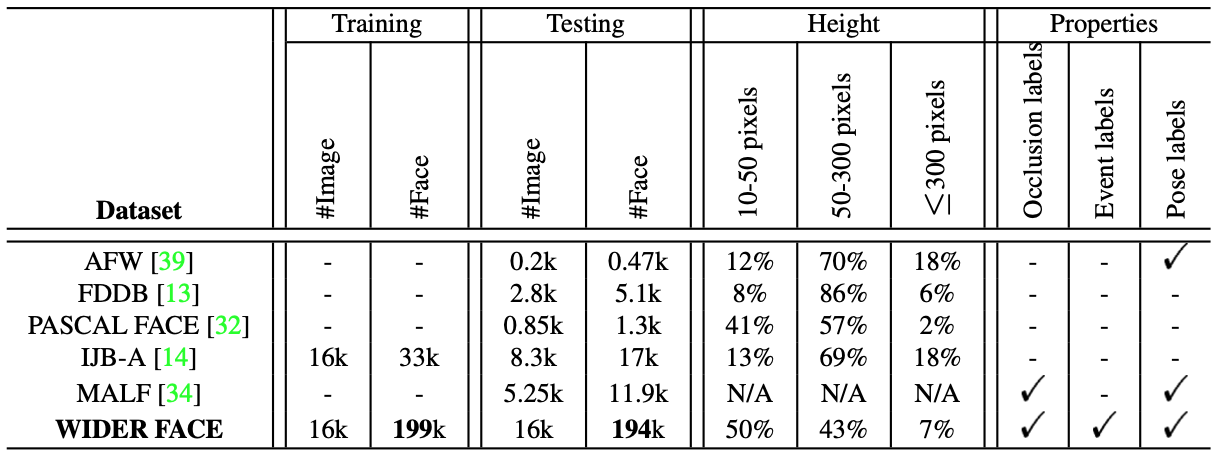
\includegraphics[width=15cm] {images/widerface_compare_1}
        \caption{So sánh về số lượng và độ đa dạng của bộ dữ liệu WIDER FACE với một số bộ dữ liệu khác (Nguồn: \cite{yang2016wider})}
        \label{fig:widerface_compare_1}
    \end{figure}

    \subsubsection*{Các thông số của bộ dữ liệu WIDER FACE}
    Bộ dữ liệu WIDER FACE bao gồm 32,203 ảnh với 393,703 hộp giới hạn\index{hộp giới hạn} của khuôn mặt với sự đa dạng về kích thước, góc quay, che chắn.
    Bộ dữ liệu WIDER FACE được chụp từ 61 khung cảnh khác nhau, trong đó, với mỗi khung cảnh, nhóm tác giả chia thành ba bộ train/val/test theo tỷ lệ 40\%/10\%/50\%.

    \noindent
    Nhóm tác giả của bộ dữ liệu WIDER FACE sử dụng mô hình EdgeBox \cite{zitnick2014edge} để chia bộ dữ liệu thành ba mức độ khó (bộ Dễ, bộ Trung bình và bộ Khó).
    Trong đó, mô hình EdgeBox đạt mức recall lần lượt tương ứng với bộ Dễ, bộ Trung bình và bộ Khó là 92\%, 76\% và 34\%.
    Mô hình EdgeBox đạt kết quả kém hơn rất nhiều trên bộ WIDER FACE so sánh với kết quả trên các bộ dữ liệu khác.

    \begin{figure}[H]
        \centering
        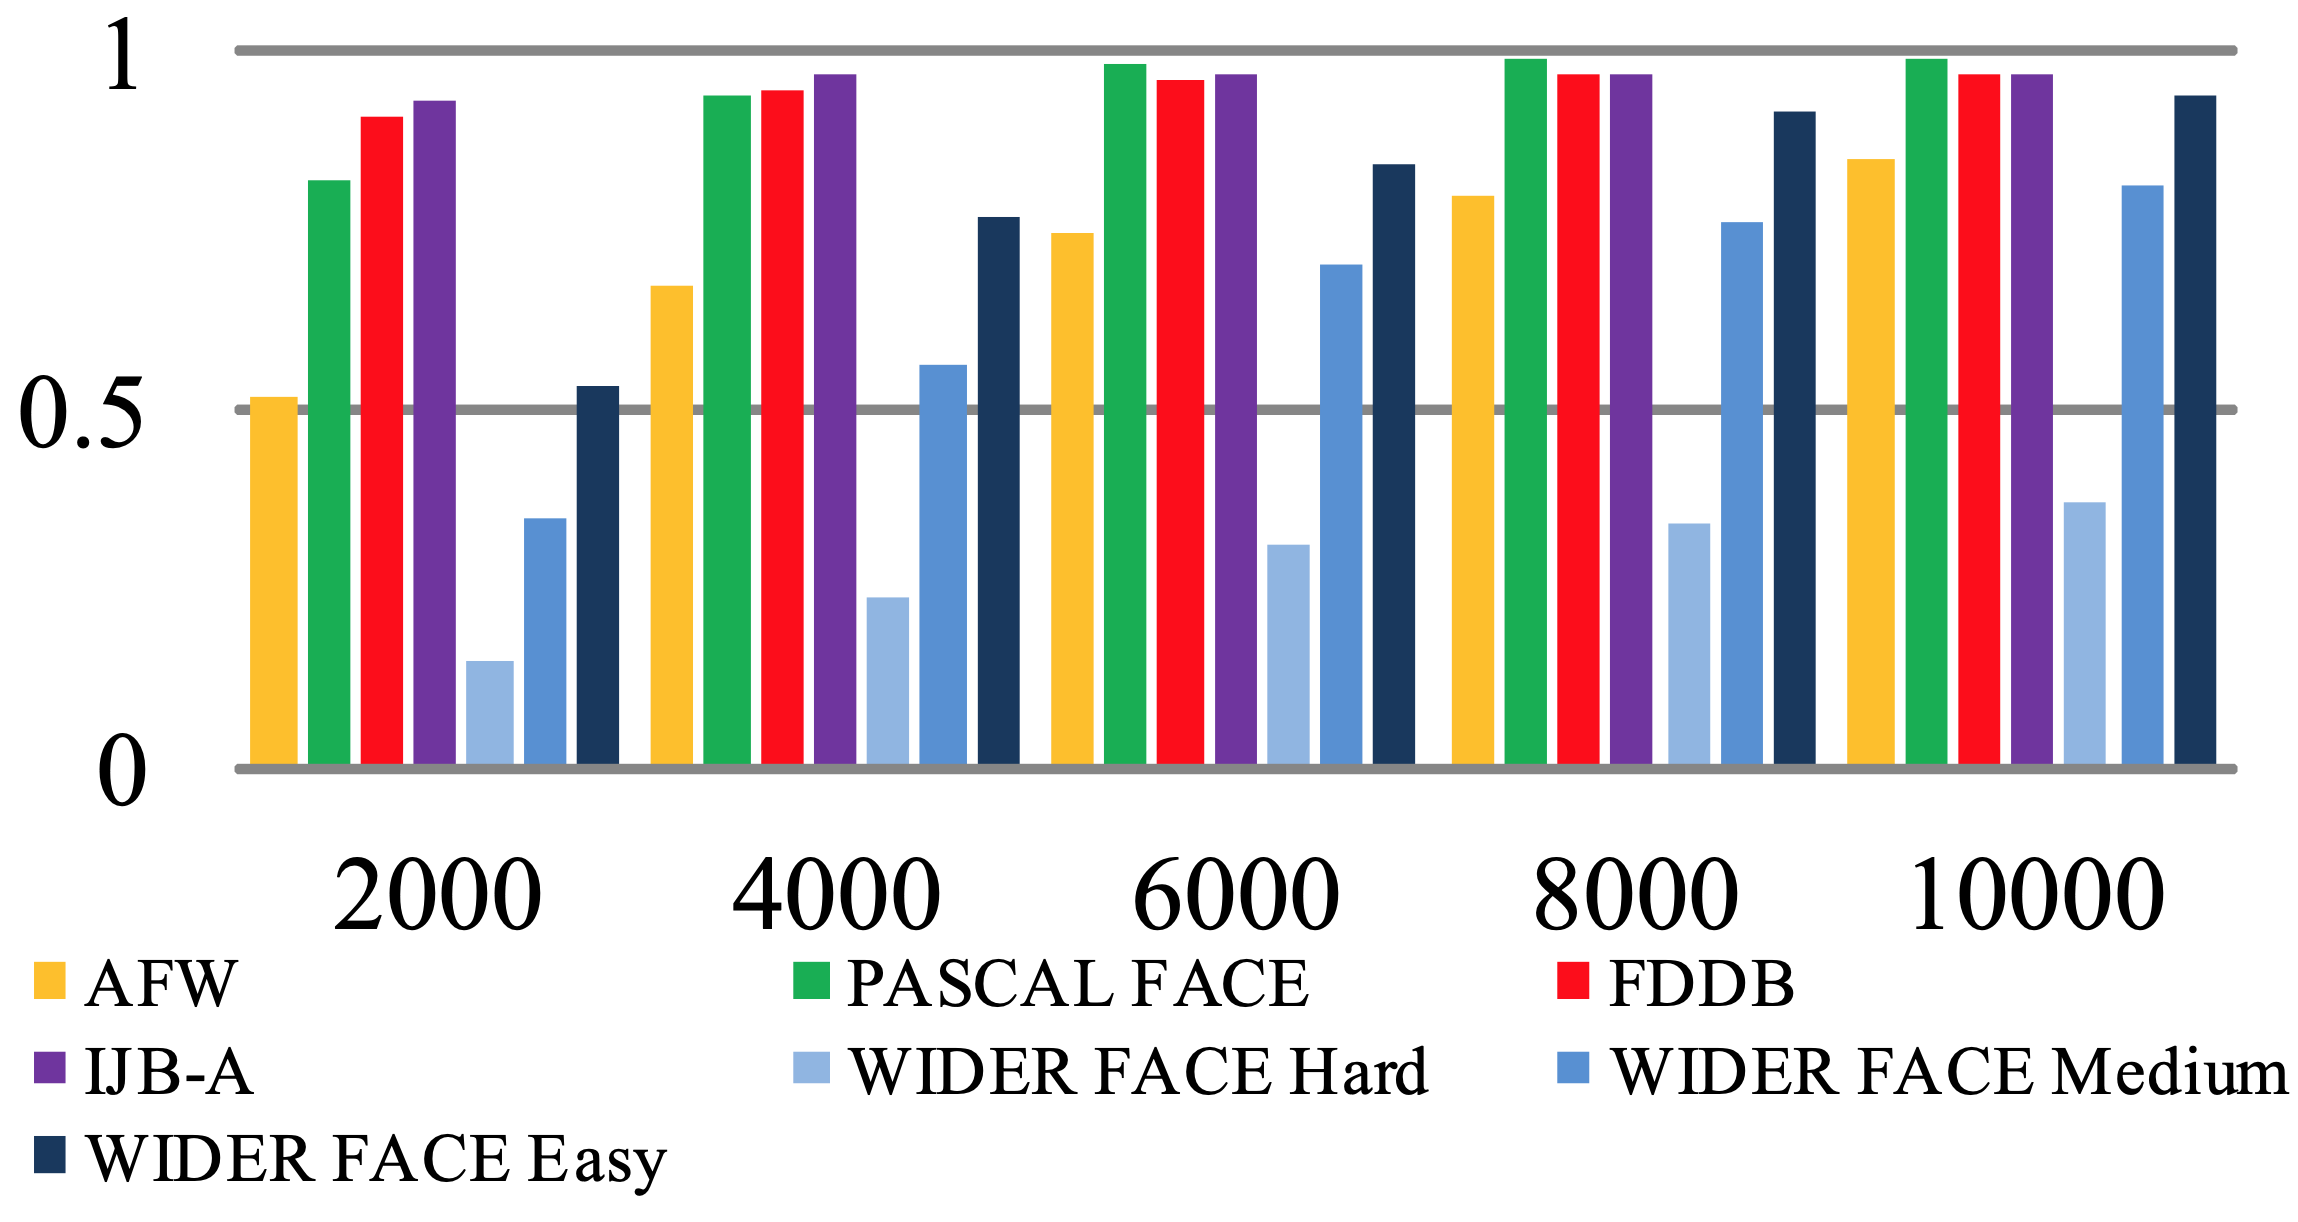
\includegraphics[width=10cm] {images/widerface_compare_2}
        \caption{So sánh độ khó của bộ dữ liệu WIDER FACE với các bộ dữ liệu khác (Nguồn: \cite{yang2016wider})}
        \label{fig:widerface_compare_2}
    \end{figure}

    \begin{figure}[H]
        \centering
        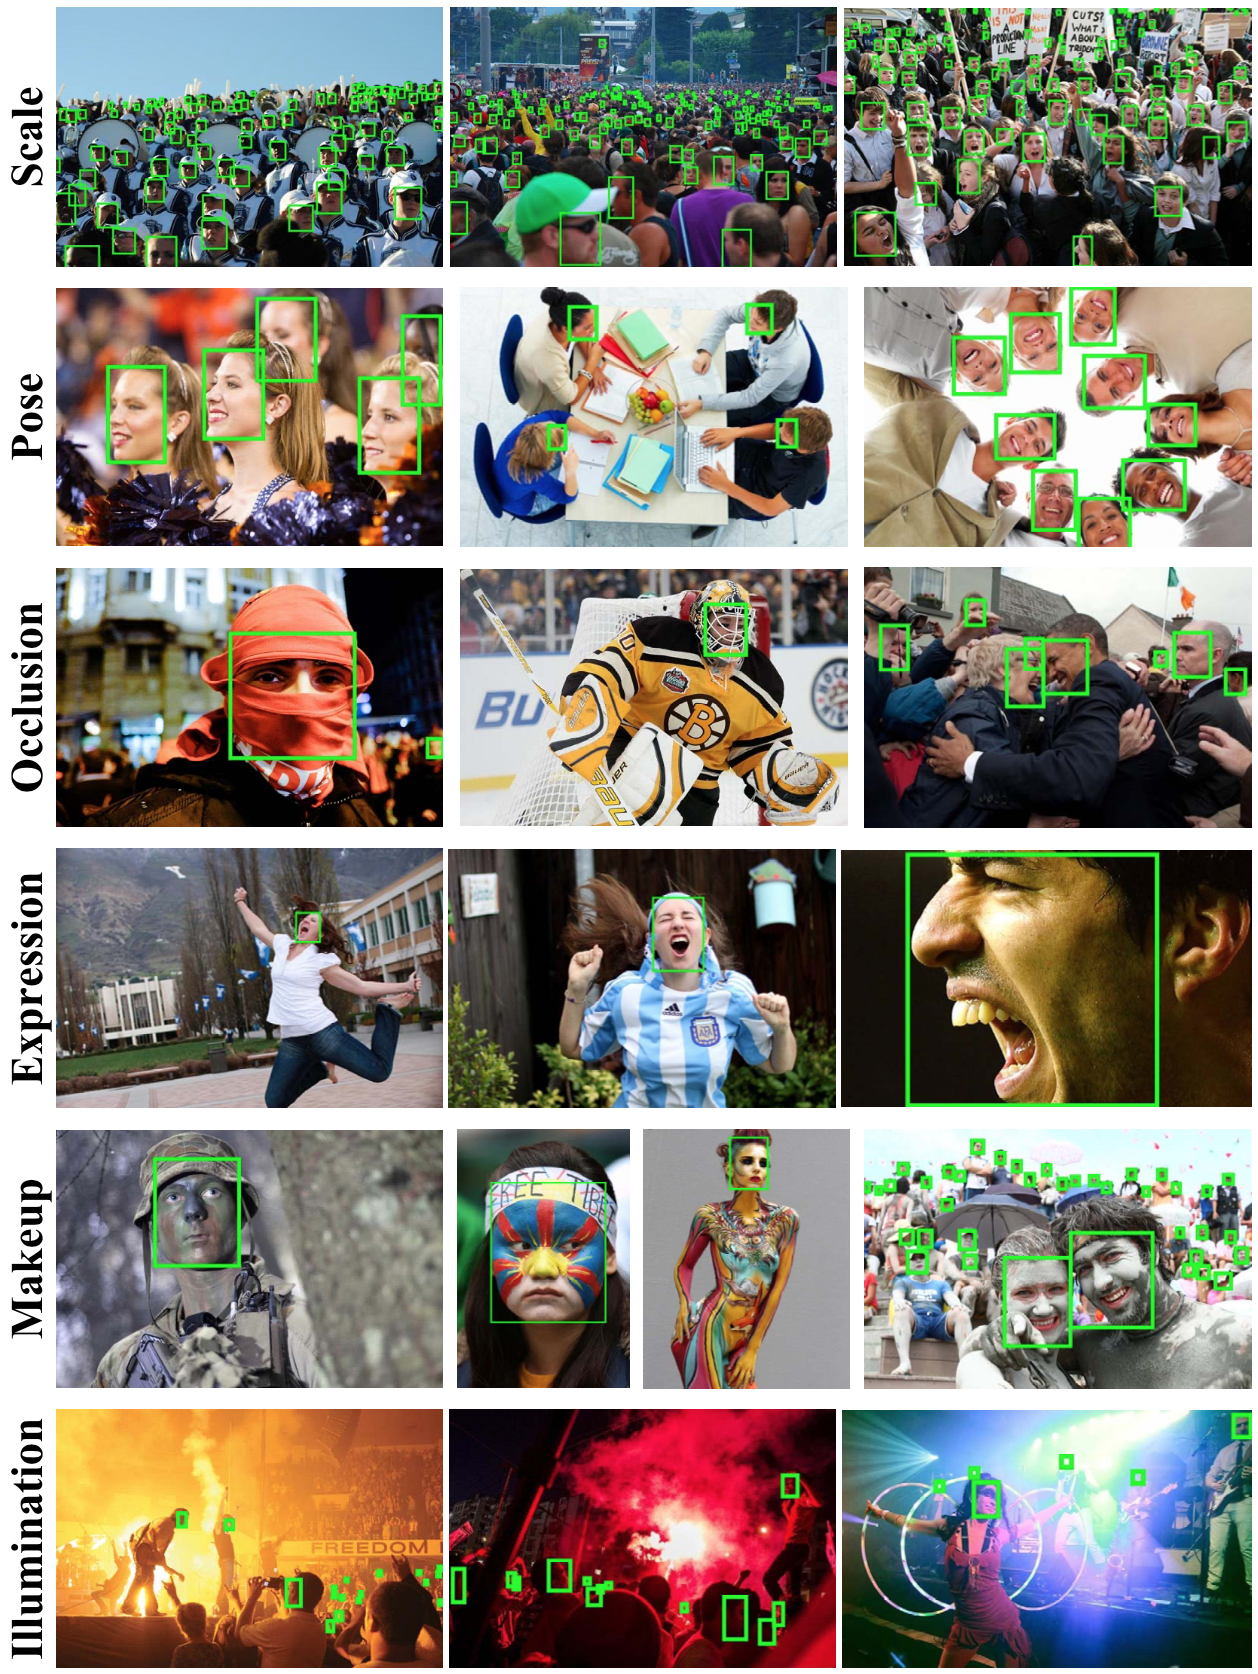
\includegraphics[width=15cm] {images/widerface_examples}
        \caption{Một số ví dụ trong bộ dữ liệu WIDER FACE (Nguồn: \cite{yang2016wider})}
        \label{fig:widerface_examples}
    \end{figure}

    \subsubsection*{Bộ dữ liệu WIDER FACE với landmarks}
    Nhóm tác giả của mô hình RetinaFace \cite{deng2020retinaface} đã bổ sung thêm vào bộ dữ liệu WIDER FACE thông tin về landmarks của các khuôn mặt bao gồm 5 điểm: tâm của mắt trái, tâm của mắt phải, đỉnh của mũi, điểm mép miệng trái và điểm mép miệng phải.

    \begin{figure}[H]
        \centering
        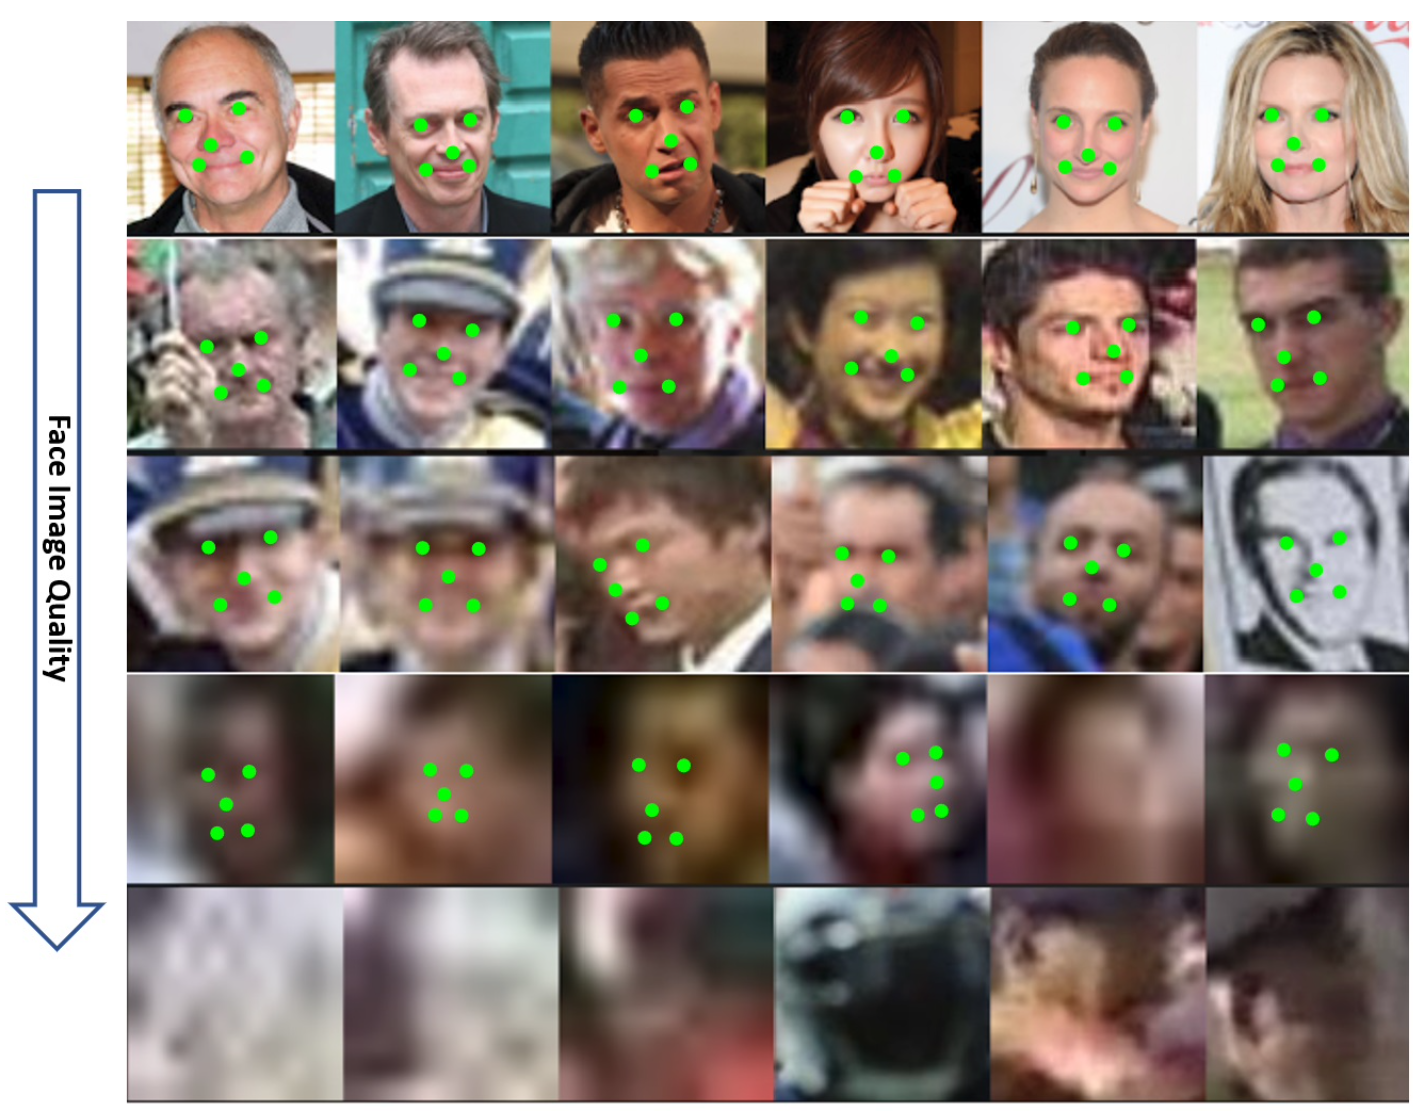
\includegraphics[width=10cm] {images/widerface_five_levels_lm_1}
        \caption{Ví dụ về mức độ khó của khuôn mặt trong việc gán landmarks (Nguồn: \cite{deng2020retinaface})}
        \label{fig:widerface_five_levels_lm_1}
    \end{figure}

    \noindent
    Dựa vào chất lượng của ảnh, nhóm tác giả đã chia bộ dữ liệu thành 5 mức độ khó: \\
    - Độ khó 1 (dễ nhất): Dễ dàng gán nhãn được 68 điểm landmarks của mặt. \\
    - Độ khó 2: Có thể gán nhãn được 68 điểm landmarks của mặt. \\
    - Độ khó 3: Dễ dàng gán nhãn được 5 điểm landmarks của mặt. \\
    - Độ khó 4: Có thể gán nhãn được 5 điểm landmarks của mặt. \\
    - Độ khó 5 (khó nhất): Chỉ có thể phân biệt được với background\index{background} của ảnh. Với các hộp giới hạn\index{hộp giới hạn} ở mức độ khó này, nhóm tác giả không gán 5 điểm landmarks. \\
    Dựa vào các mức độ khó nói trên, nhóm tác giả của RetinaFace đã gán landmarks cho các khuôn mặt trong hai tập dữ liệu huấn luyện và val, tương ứng 84.6k mặt cho tập huấn luyện và 18.5k mặt cho bộ val.

    \begin{figure}[H]
        \centering
        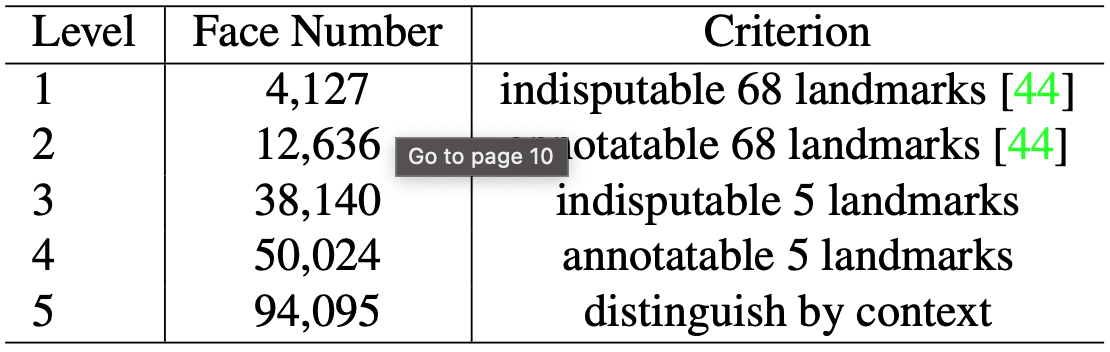
\includegraphics[width=11cm] {images/widerface_five_levels_lm_2}
        \caption{Các thông số của độ khó của khuôn mặt trong việc gán landmarks (Nguồn: \cite{deng2020retinaface})}
        \label{fig:widerface_five_levels_lm_2}
    \end{figure}

    \subsubsection*{Vấn đề tồn đọng của bộ dữ liệu WIDER FACE}
    Ở thời điểm ra mắt, bộ dữ liệu WIDER FACE thật sự là một bước tiến về dữ liệu cho bài toán nhận diện khuôn mặt bởi số lượng và sự đa dạng.
    Tuy nhiên, cho đến nay, kích thước như ảnh trong bộ WIDER FACE khoảng 1000 - 1500 điểm ảnh\index{điểm ảnh} không còn là kích thước lớn nữa.
    Điều này là rào cản cho giới nghiên cứu khi phát triển các mô hình giải quyết bài toán nhận diện khuôn mặt trong ảnh chất lượng cao.
}
    \widerface

    \begin{figure}[H]
        \centering
        \subfigure[]{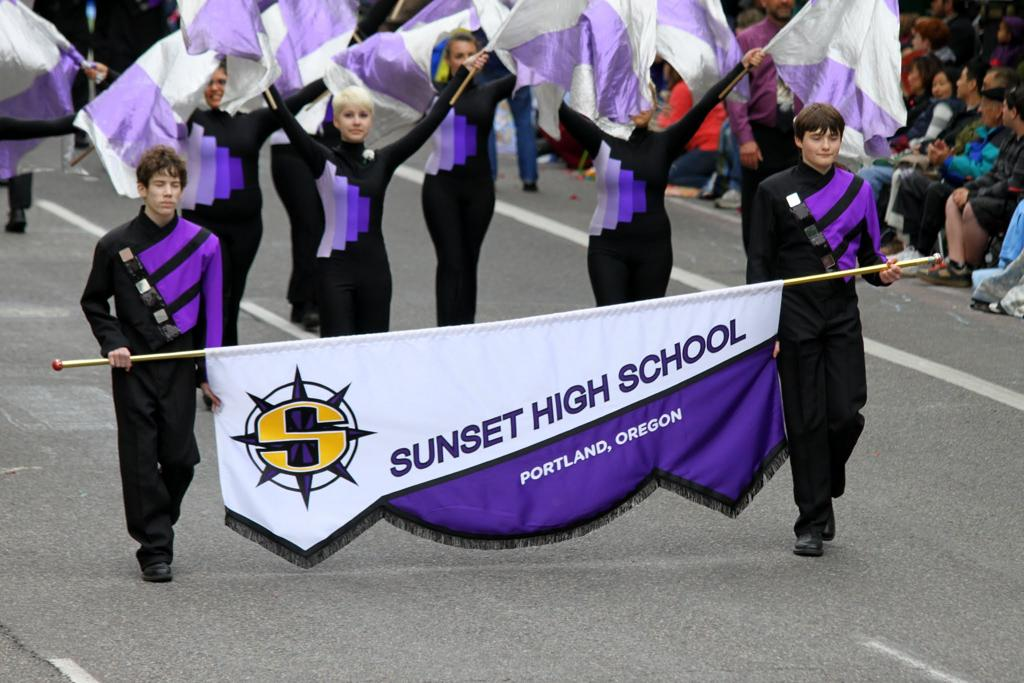
\includegraphics[width=7.3cm]{images/widerface_highres_1}}
        \subfigure[]{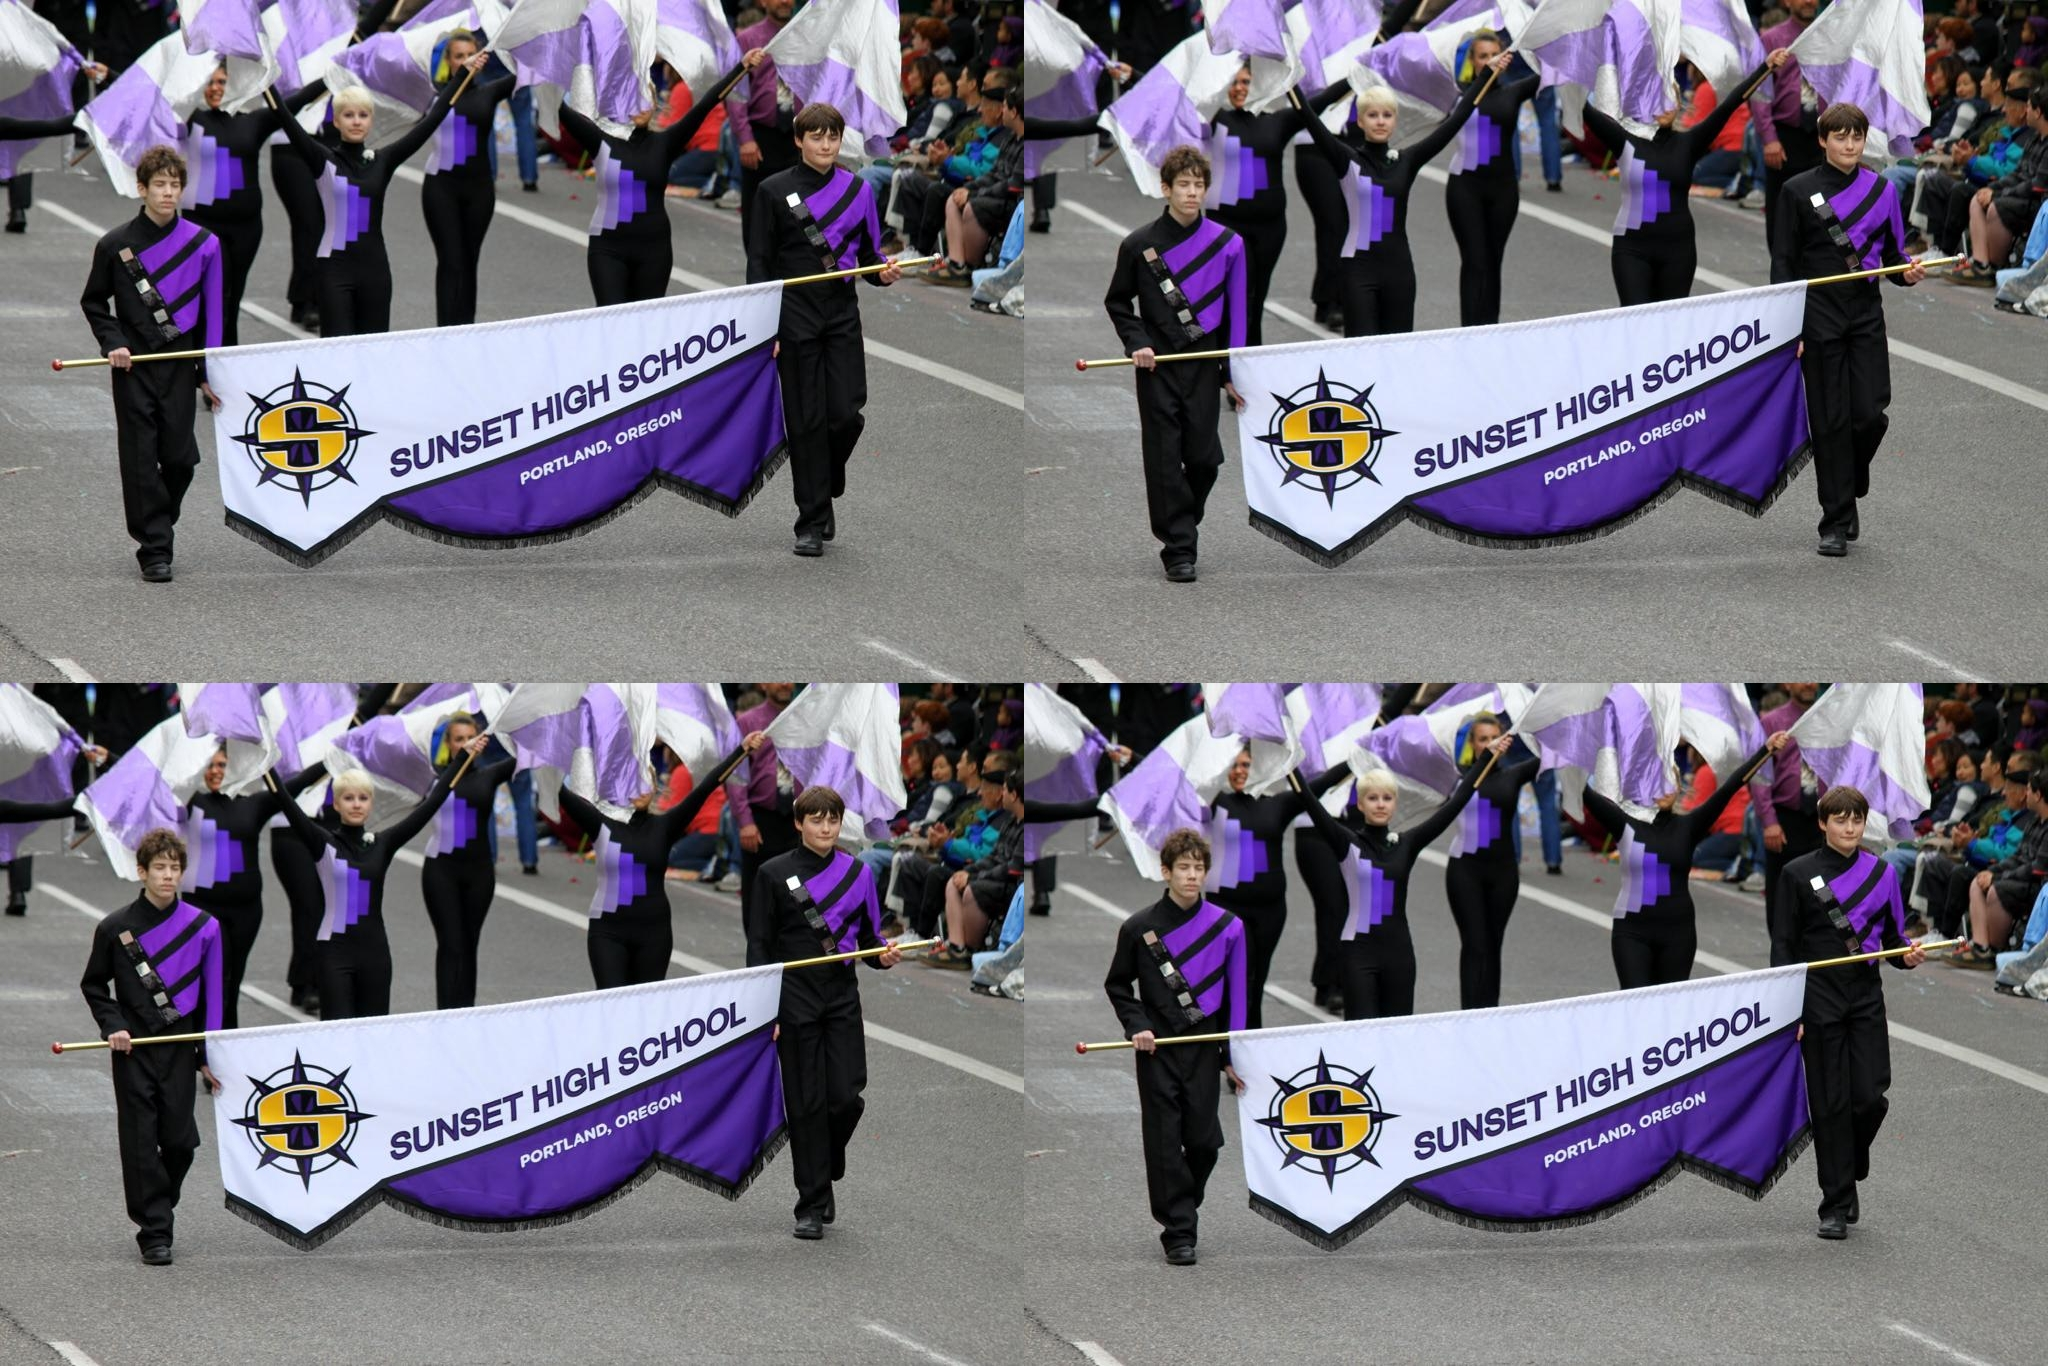
\includegraphics[width=7.3cm]{images/widerface_highres_2}}
        \subfigure[]{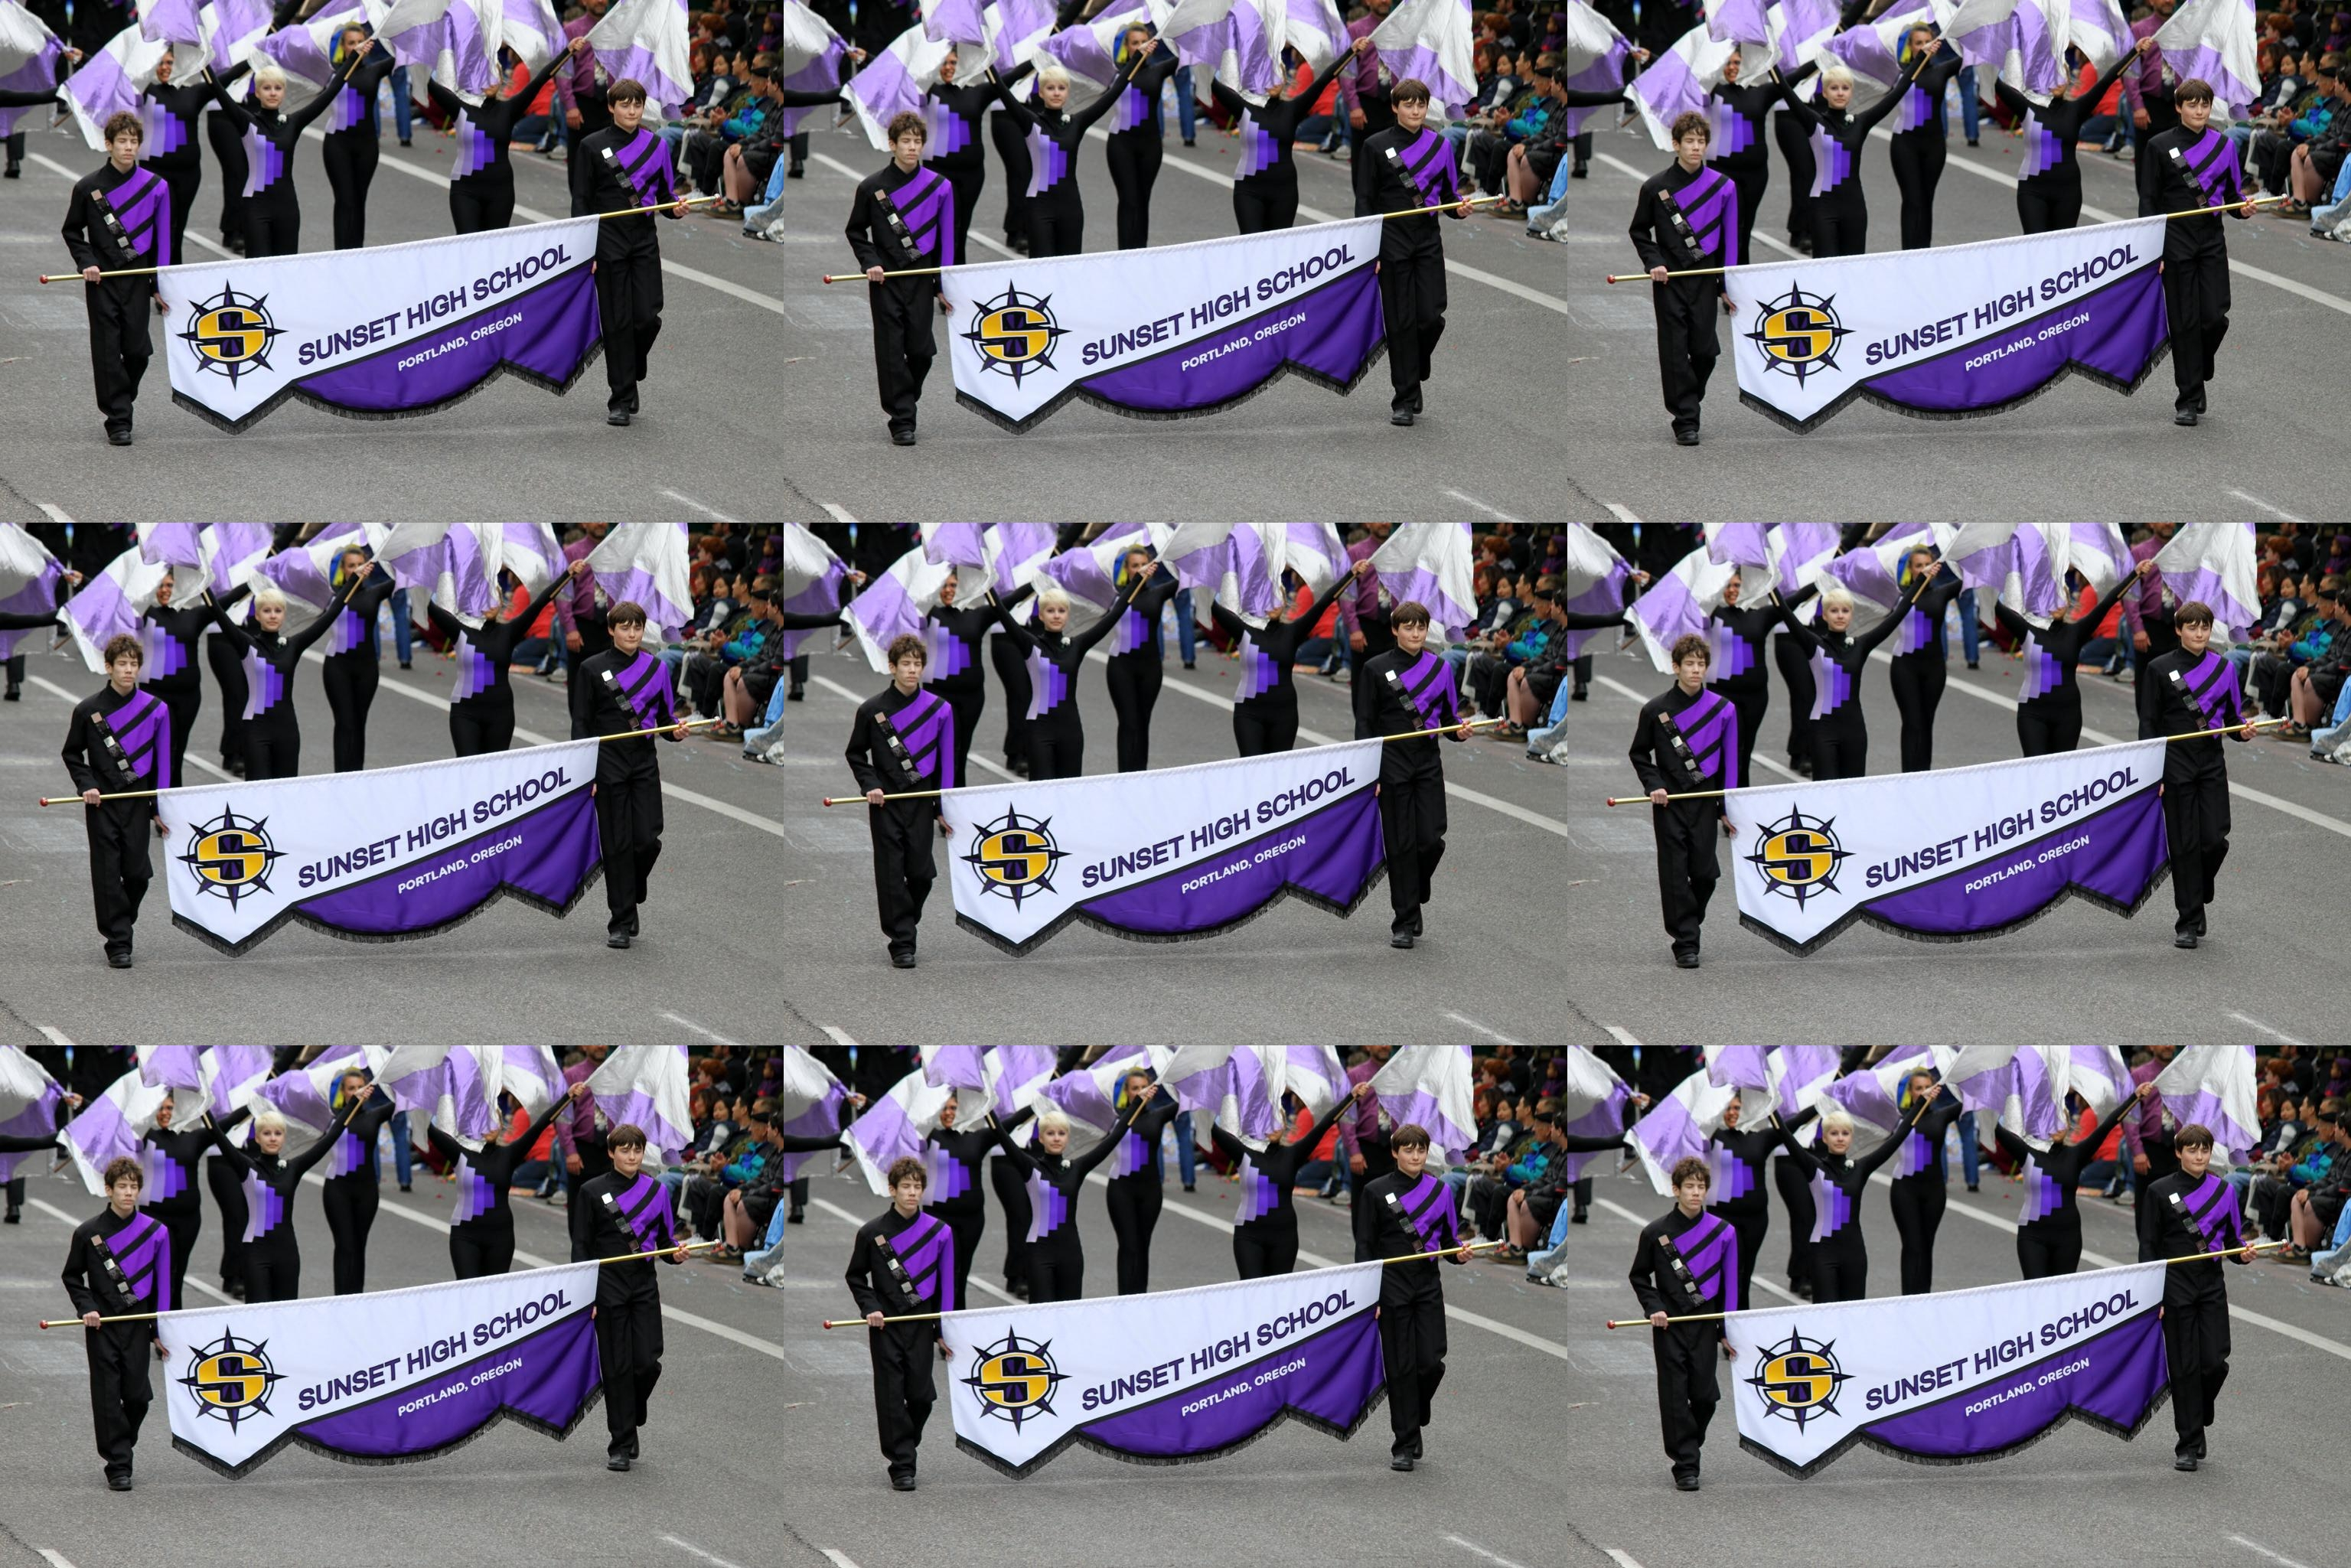
\includegraphics[width=10cm]{images/widerface_highres_3}}
        \caption{Một ví dụ ảnh trong bộ dữ liệu WIDER FACE \cite{yang2016wider} (a) so sánh với bộ dữ liệu WIDER FACE kích thước lớn dạng lưới $2 X 2$ (b) và $3 X 3$ (c)}
        \label{fig:widerface_4k_example}
    \end{figure}

    \subsection{Bộ dữ liệu WIDER FACE kích thước lớn}
    \def\widerfacefourk{
    Kế thừa những điểm mạnh về sự đa dạng của khuôn mặt trong bộ dữ liệu WIDER FACE \cite{yang2016wider}, tôi đề xuất một phương pháp xây dựng bộ dữ liệu WIDER FACE kích thước lớn gồm có nhiều ảnh có độ phân giải cao, giúp đánh giá khách quan độ chính xác và tốc độ của các mô hình giải bài toán nhận diện khuôn mặt với ảnh chất lượng cao.

    \begin{figure}[H]
        \centering
        \subfigure[]{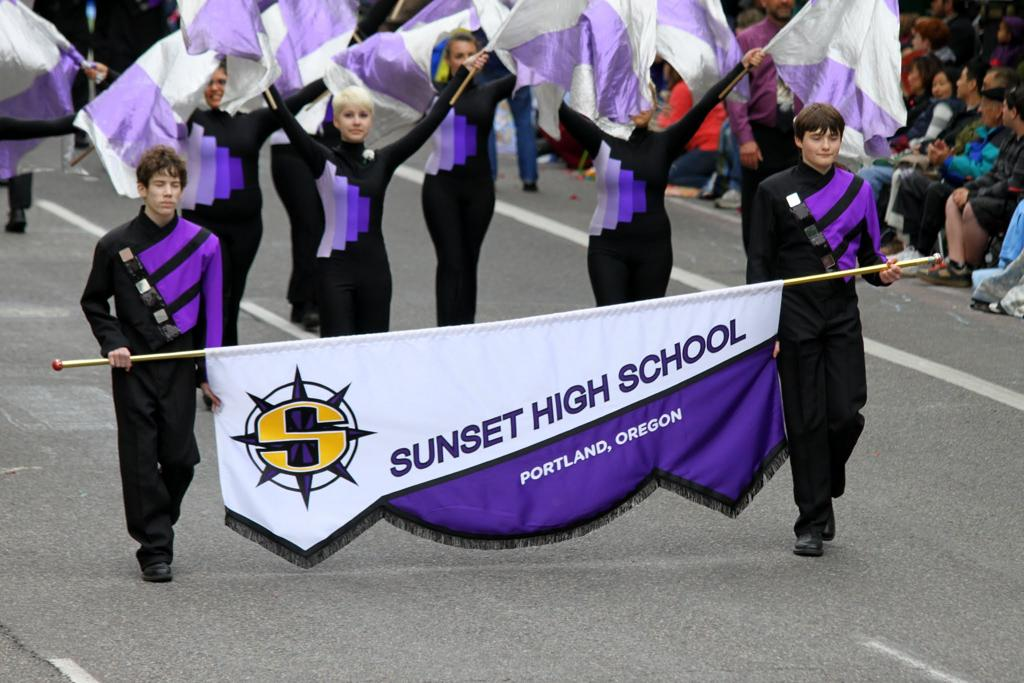
\includegraphics[width=7.3cm]{images/widerface_highres_1}}
        \subfigure[]{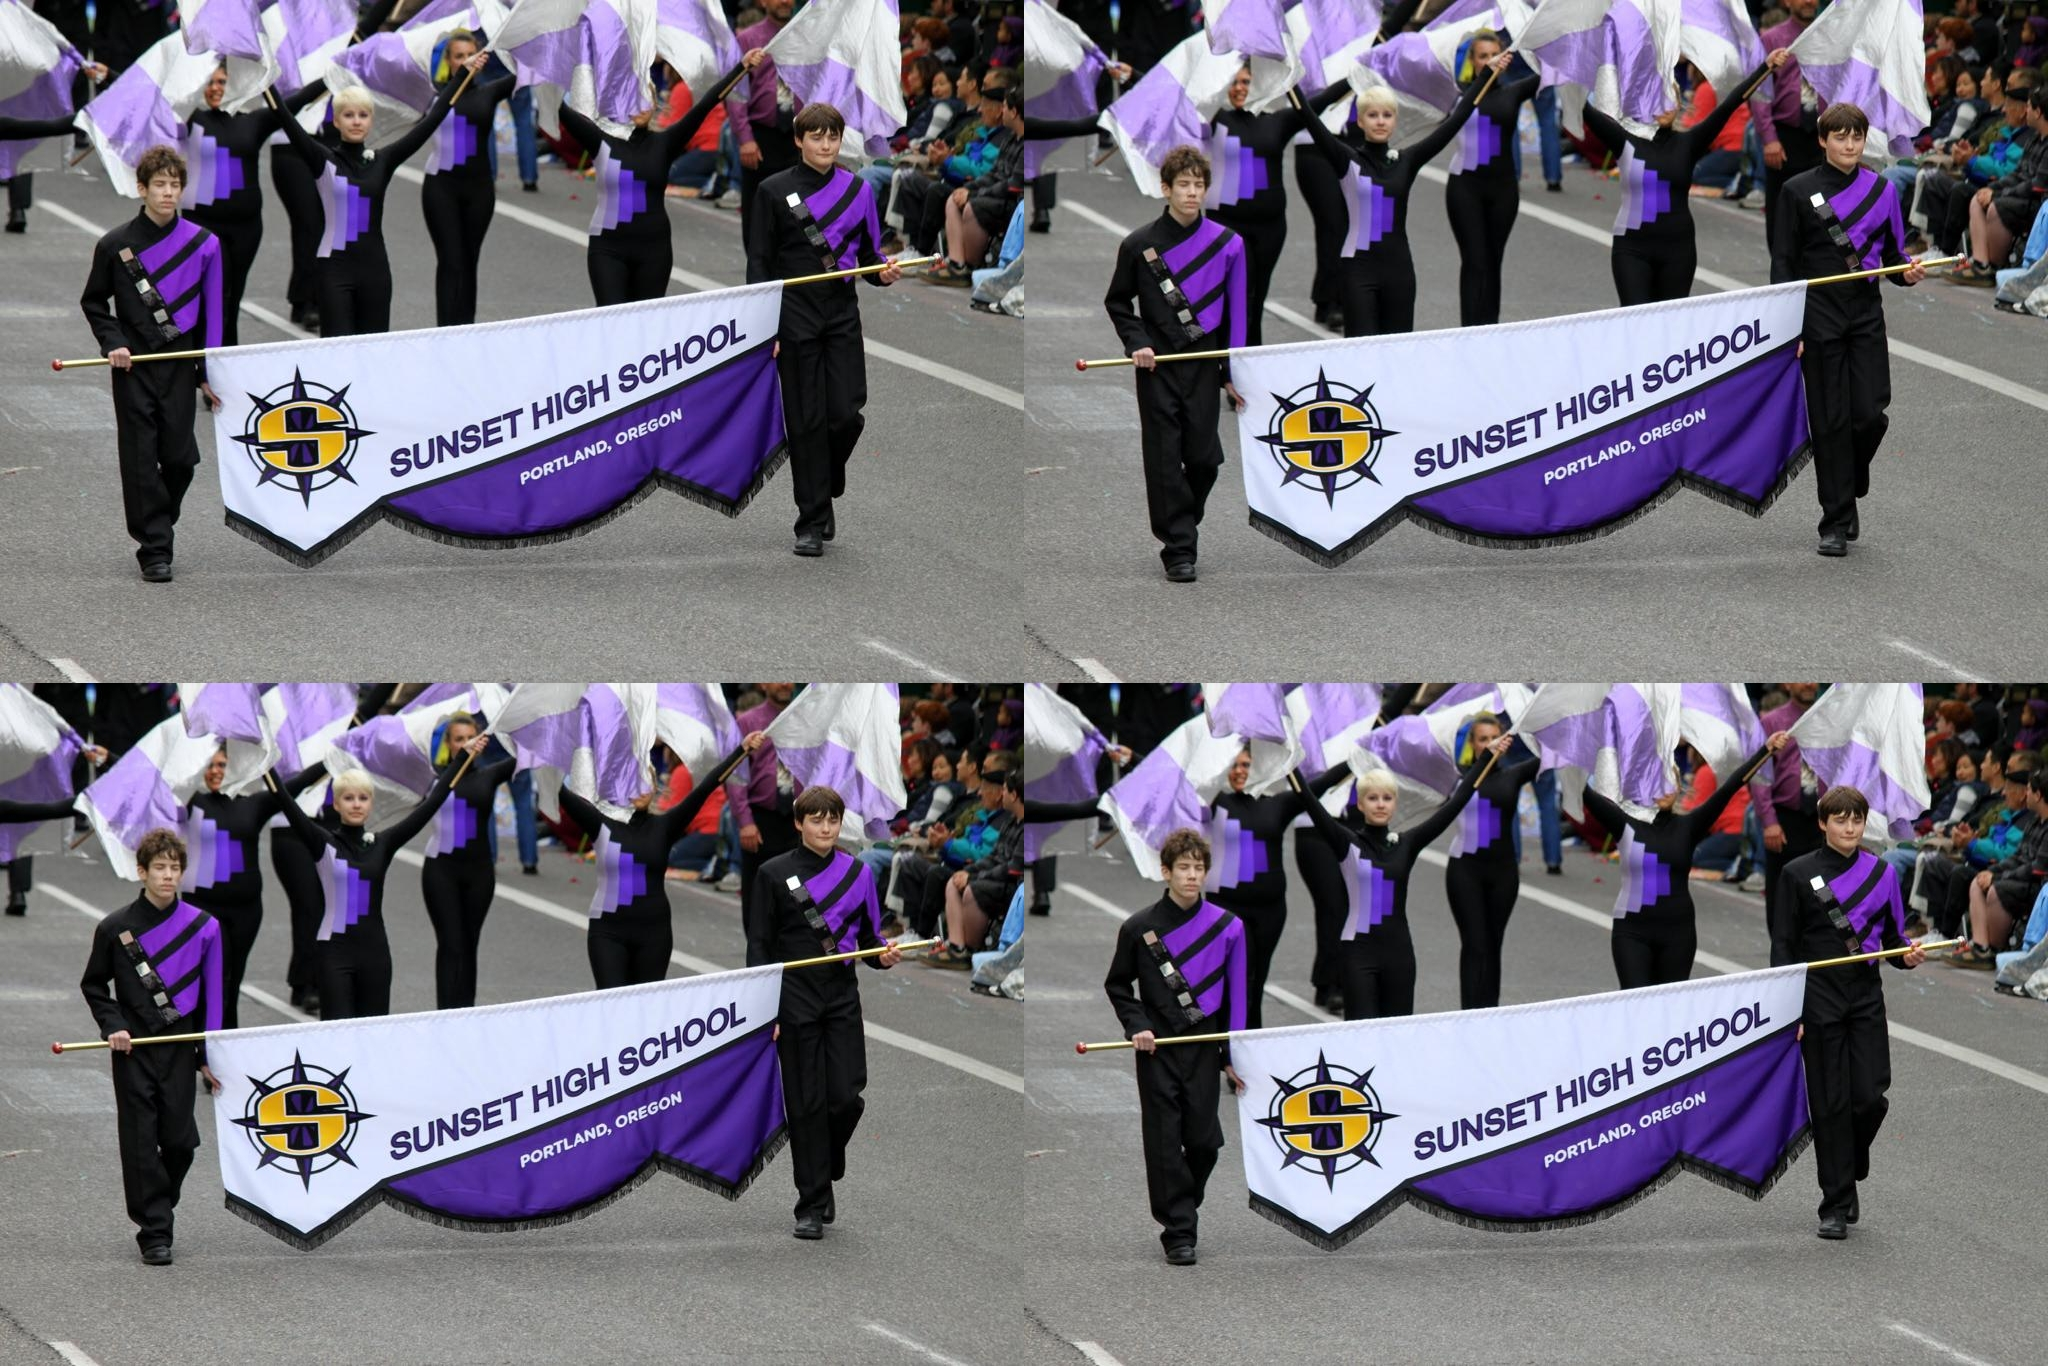
\includegraphics[width=7.3cm]{images/widerface_highres_2}}
        \subfigure[]{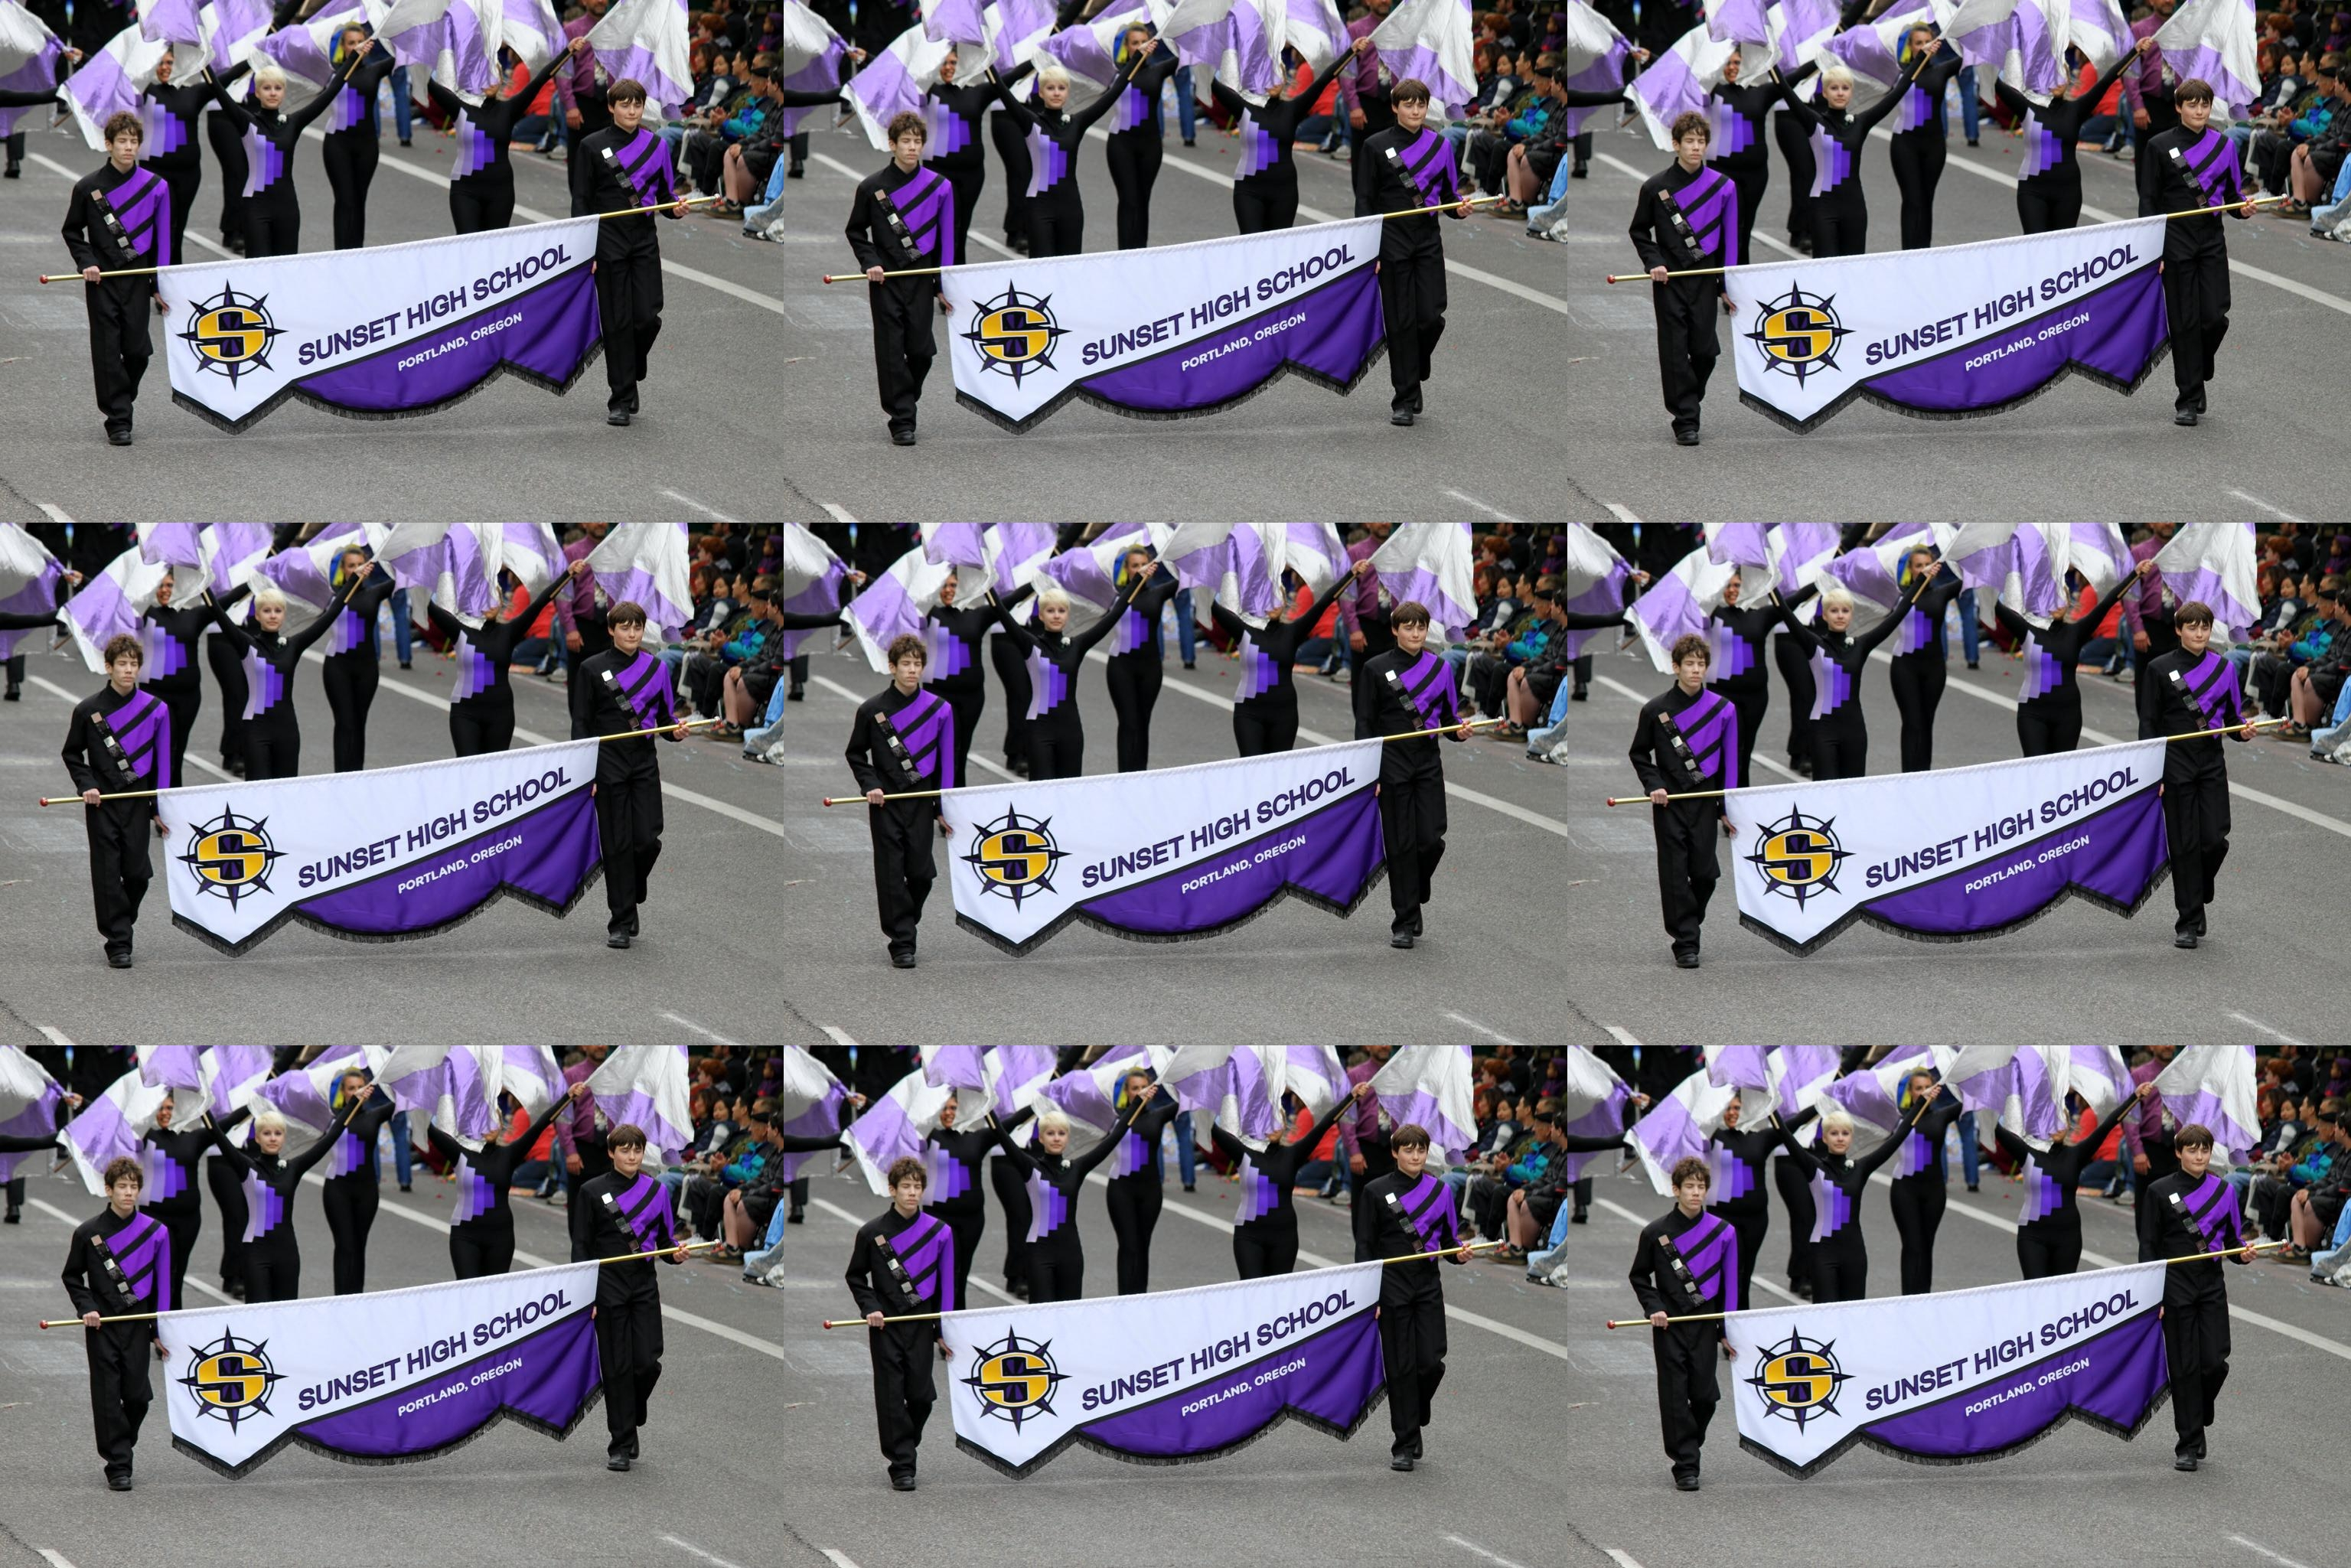
\includegraphics[width=9.4cm]{images/widerface_highres_3}}
        \caption{Một ví dụ ảnh trong bộ dữ liệu WIDER FACE \cite{yang2016wider} (a) so sánh với bộ dữ liệu WIDER FACE kích thước lớn dạng lưới $2 X 2$ (b) và $3 X 3$ (c)}
        \label{fig:widerface_4k_example}
    \end{figure}

    \subsubsection*{Ý tưởng xây dựng bộ dữ liệu WIDER FACE kích thước lớn}
    Nhằm tận dụng hết những điểm mạnh như tỷ lệ kích thước, kiểu dáng, biểu cảm, che chắn, góc quay và ánh sáng của bộ dữ liệu WIDER FACE, tôi không tác động gì đến dữ liệu ảnh của bộ dữ liệu WIDER FACE mà chỉ nối chúng lại với nhau theo dạng lưới nhằm tạo ra bộ dữ liệu ảnh có kích thước lớn hơn.
    Với số lượng cũng như độ đa dạng của khuôn mặt được giữ nguyên của bộ dữ liệu WIDER FACE, nhưng với kích thước ảnh lớn hơn, bộ dữ liệu WIDER FACE kích thước lớn sẽ đánh giá tốt khả năng của các mô hình nhận diện khuôn mặt, không chỉ ở độ chính xác, mà còn ở thời gian chạy cũng như khối lượng bộ nhớ cần dùng.

    \noindent
    Trong khuôn khổ của luận văn, tôi chỉ xây dựng các bộ dữ liệu WIDER FACE kích thước lớn với dạng lưới có kích thước $2 X 2$, và $3 X 3$, tuy nhiên, ý tưởng xây dựng bộ dữ liệu WIDER FACE kích thước lớn này hoàn toàn có thể áp dụng với các kích thước lưới lớn hơn $n X n$ nhằm tạo ra bộ dữ liệu ảnh có kích thước lớn hơn nữa.

    \begin{figure}[H]
        \centering
        \subfigure[]{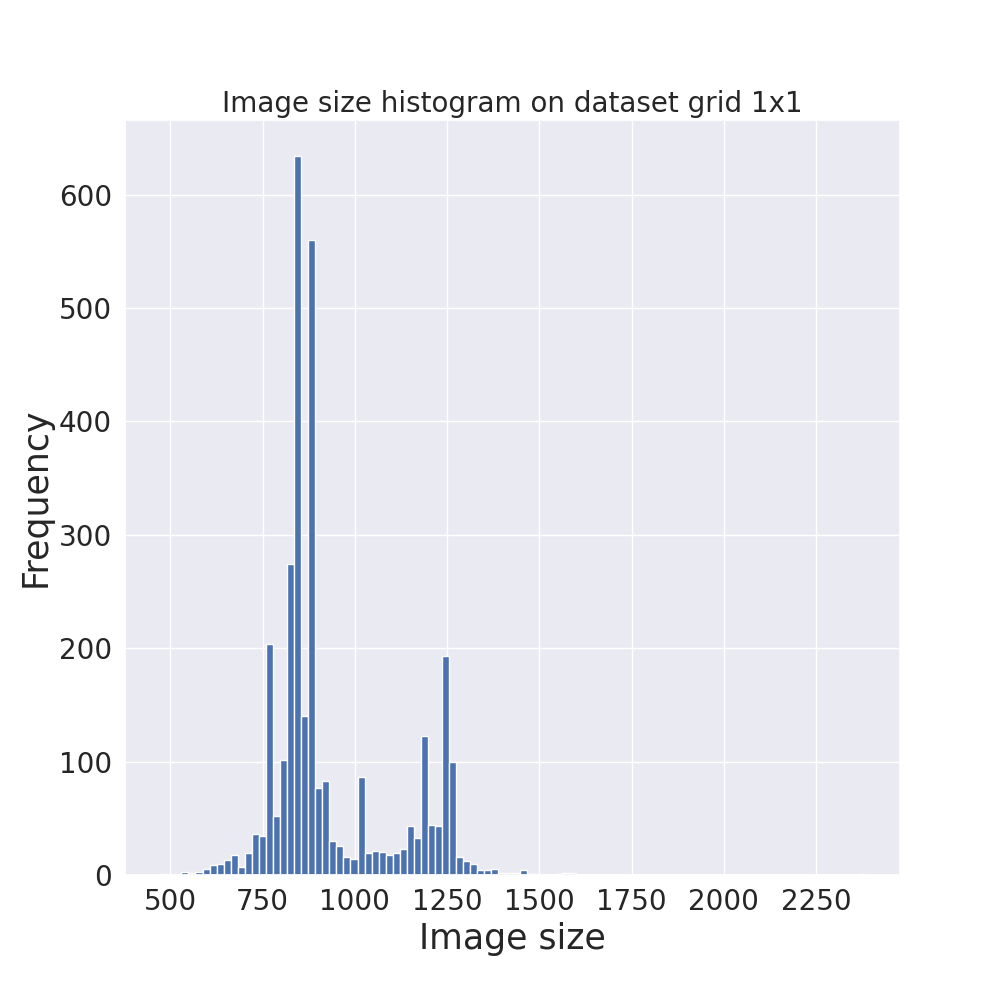
\includegraphics[width=7.3cm, trim={0.5cm 0.5cm 3cm 2cm}, clip]{images/widerface_nk_img_size_1K}}
        \subfigure[]{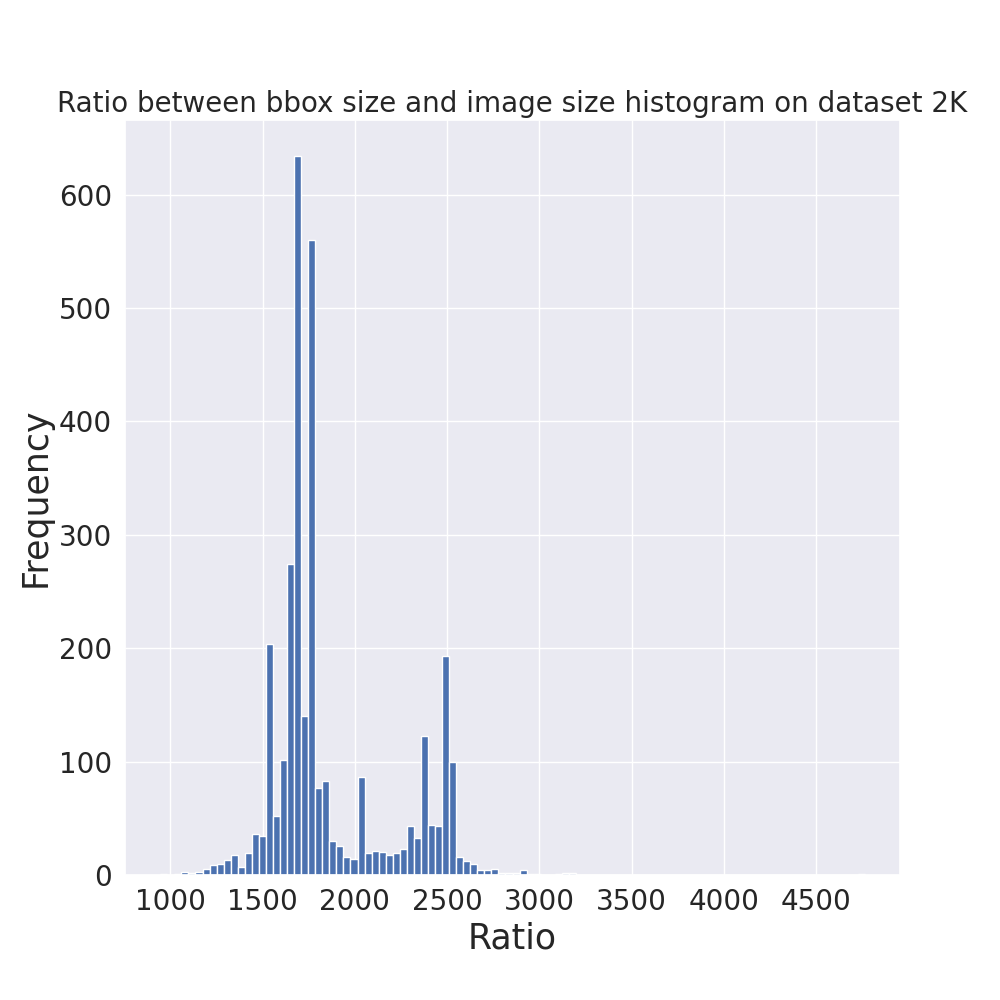
\includegraphics[width=7.3cm, trim={0.5cm 0.5cm 3cm 2cm}, clip]{images/widerface_nk_img_size_2K}}
        \subfigure[]{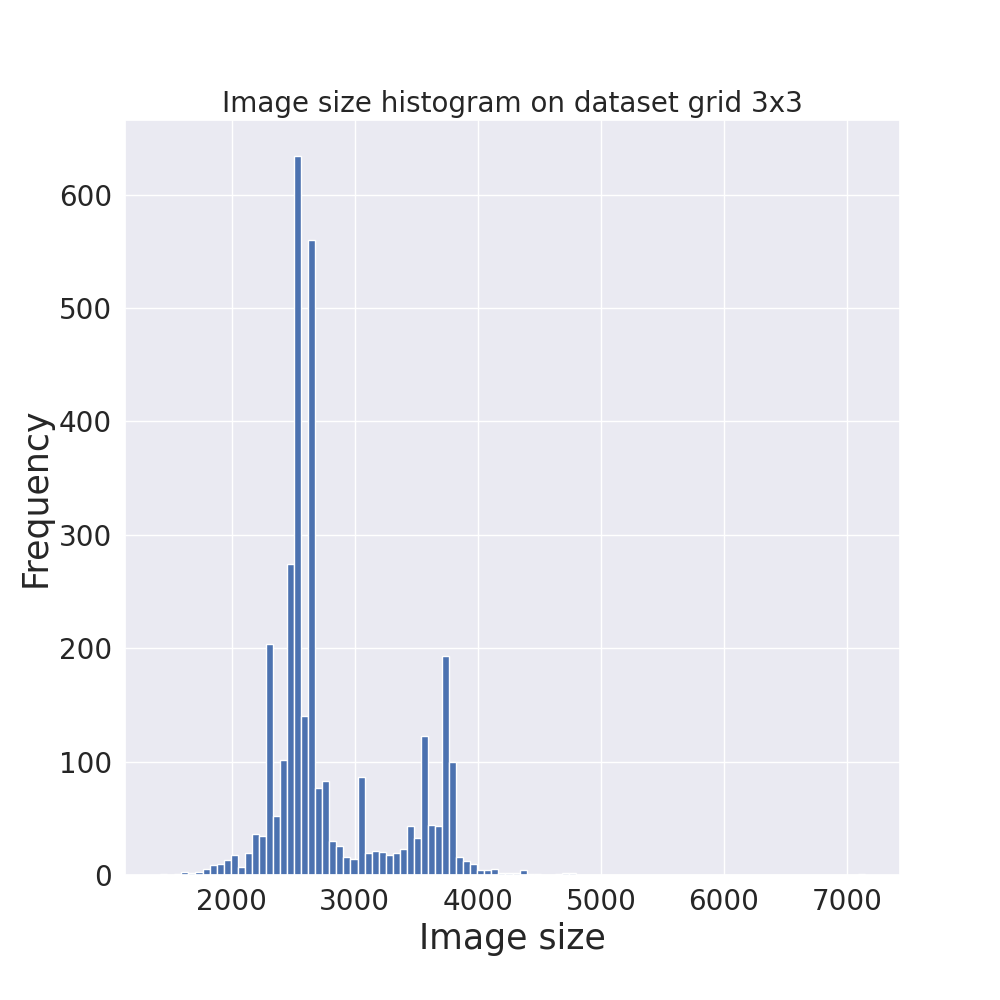
\includegraphics[width=7.3cm, trim={0.5cm 0.5cm 3cm 2cm}, clip]{images/widerface_nk_img_size_3K}}
        \caption{Phân phối về kích thước ảnh trong bộ dữ liệu WIDER FACE \cite{yang2016wider} (a) so sánh với bộ dữ liệu WIDER FACE kích thước lớn dạng lưới $2 X 2$ (b) và $3 X 3$ (c)}
        \label{fig:widerface_4k_img_size}
    \end{figure}

    \subsubsection*{Các thông số của bộ dữ liệu WIDER FACE kích thước lớn}
    Bộ dữ liệu WIDER FACE kích thước lớn, đúng với mục đích ra đời, đã làm tăng kích thước dữ liệu ảnh đáng kể.
    So sánh với bộ dữ liệu WIDER FACE với kích thước ảnh trung bình nằm trong khoảng từ 750 đến 1250 điểm ảnh mỗi chiều, bộ dữ liệu WIDER FACE kích thước lớn đã tăng kích thước ảnh trung bình từ 1500 đến 2500 điểm ảnh mỗi chiều đối với dạng lưới $2 X 2$ và 2200 đến 4000 điểm ảnh mỗi chiều đối với dạng lưới $3 X 3$.

    \noindent
    Hơn nữa, kích thước ảnh tối đa trên bộ dữ liệu WIDER FACE kích thước lớn cũng được cải thiện, so sánh với kích thước 2250 điểm ảnh của bộ dữ liệu WIDER FACE, bộ dữ liệu WIDER FACE kích thước lớn có kích thước ảnh tối đa là 4500 điểm ảnh với dạng lưới $2 X 2$ và 7000 điểm ảnh với dạng lưới $3 X 3$.

    \begin{figure}[H]
        \centering
        \subfigure[]{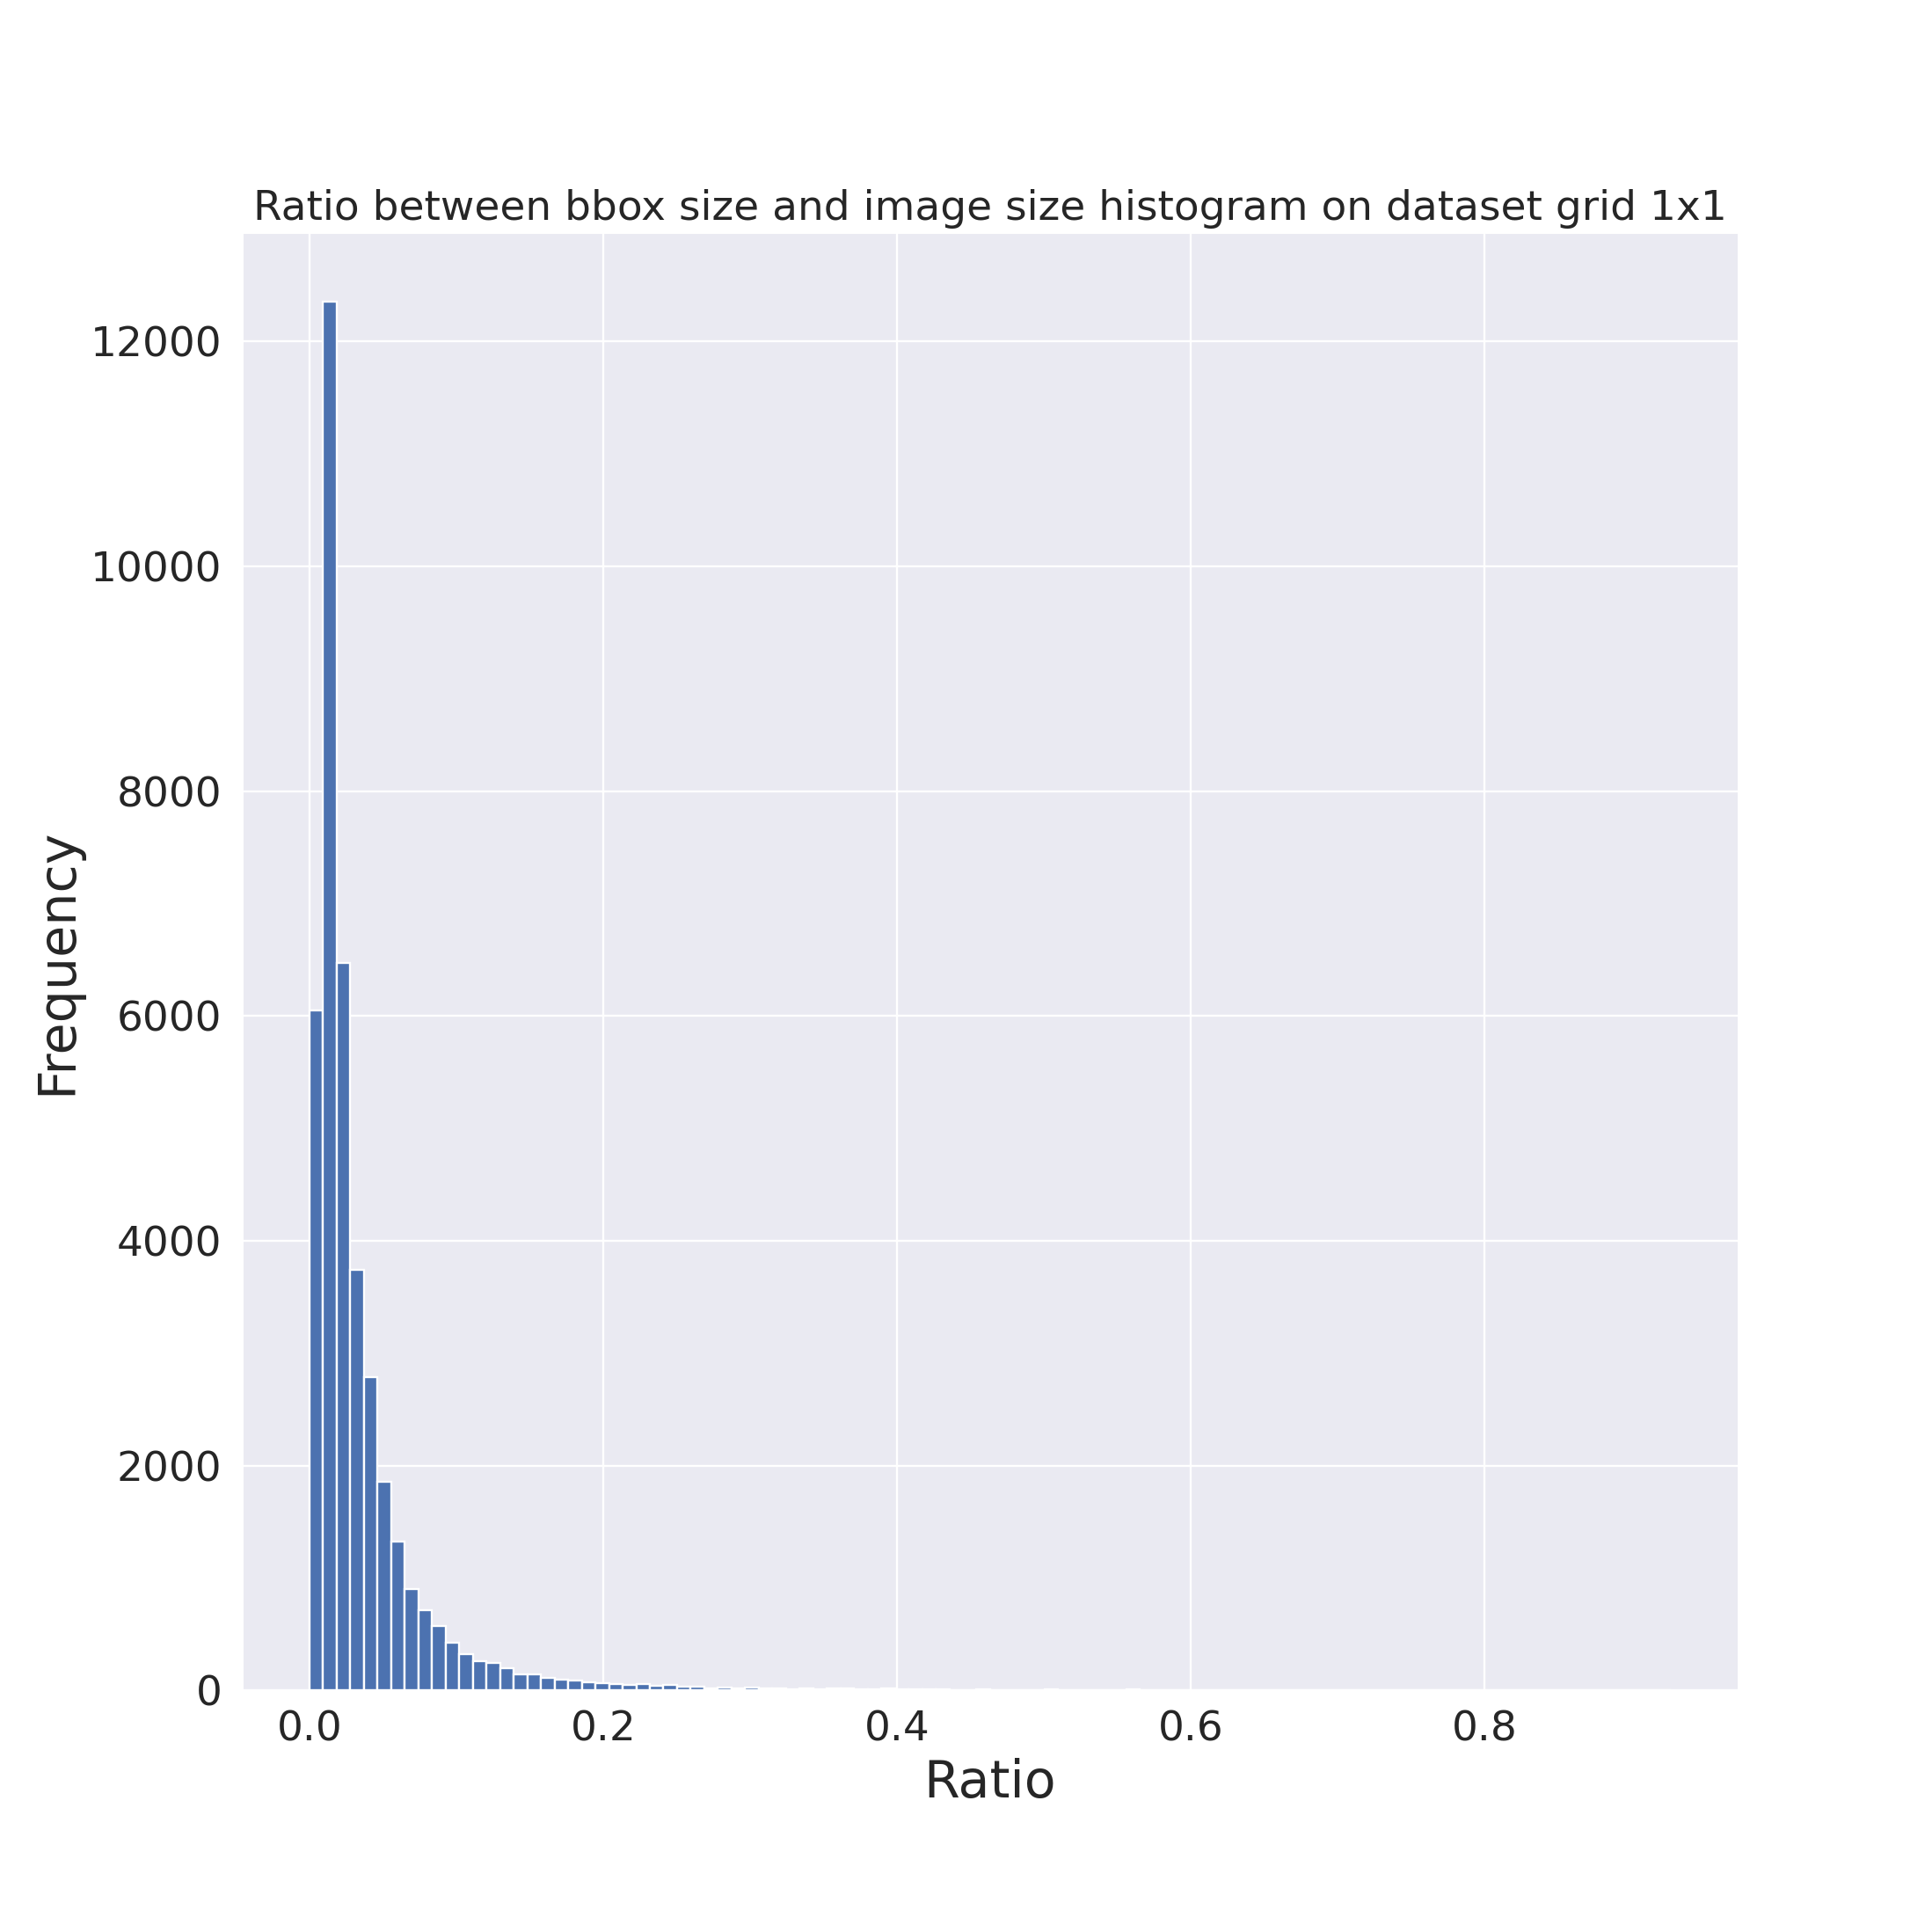
\includegraphics[width=7.3cm, trim={0.5cm 0.5cm 3cm 3cm}, clip]{images/widerface_nk_scale_1K}}
        \subfigure[]{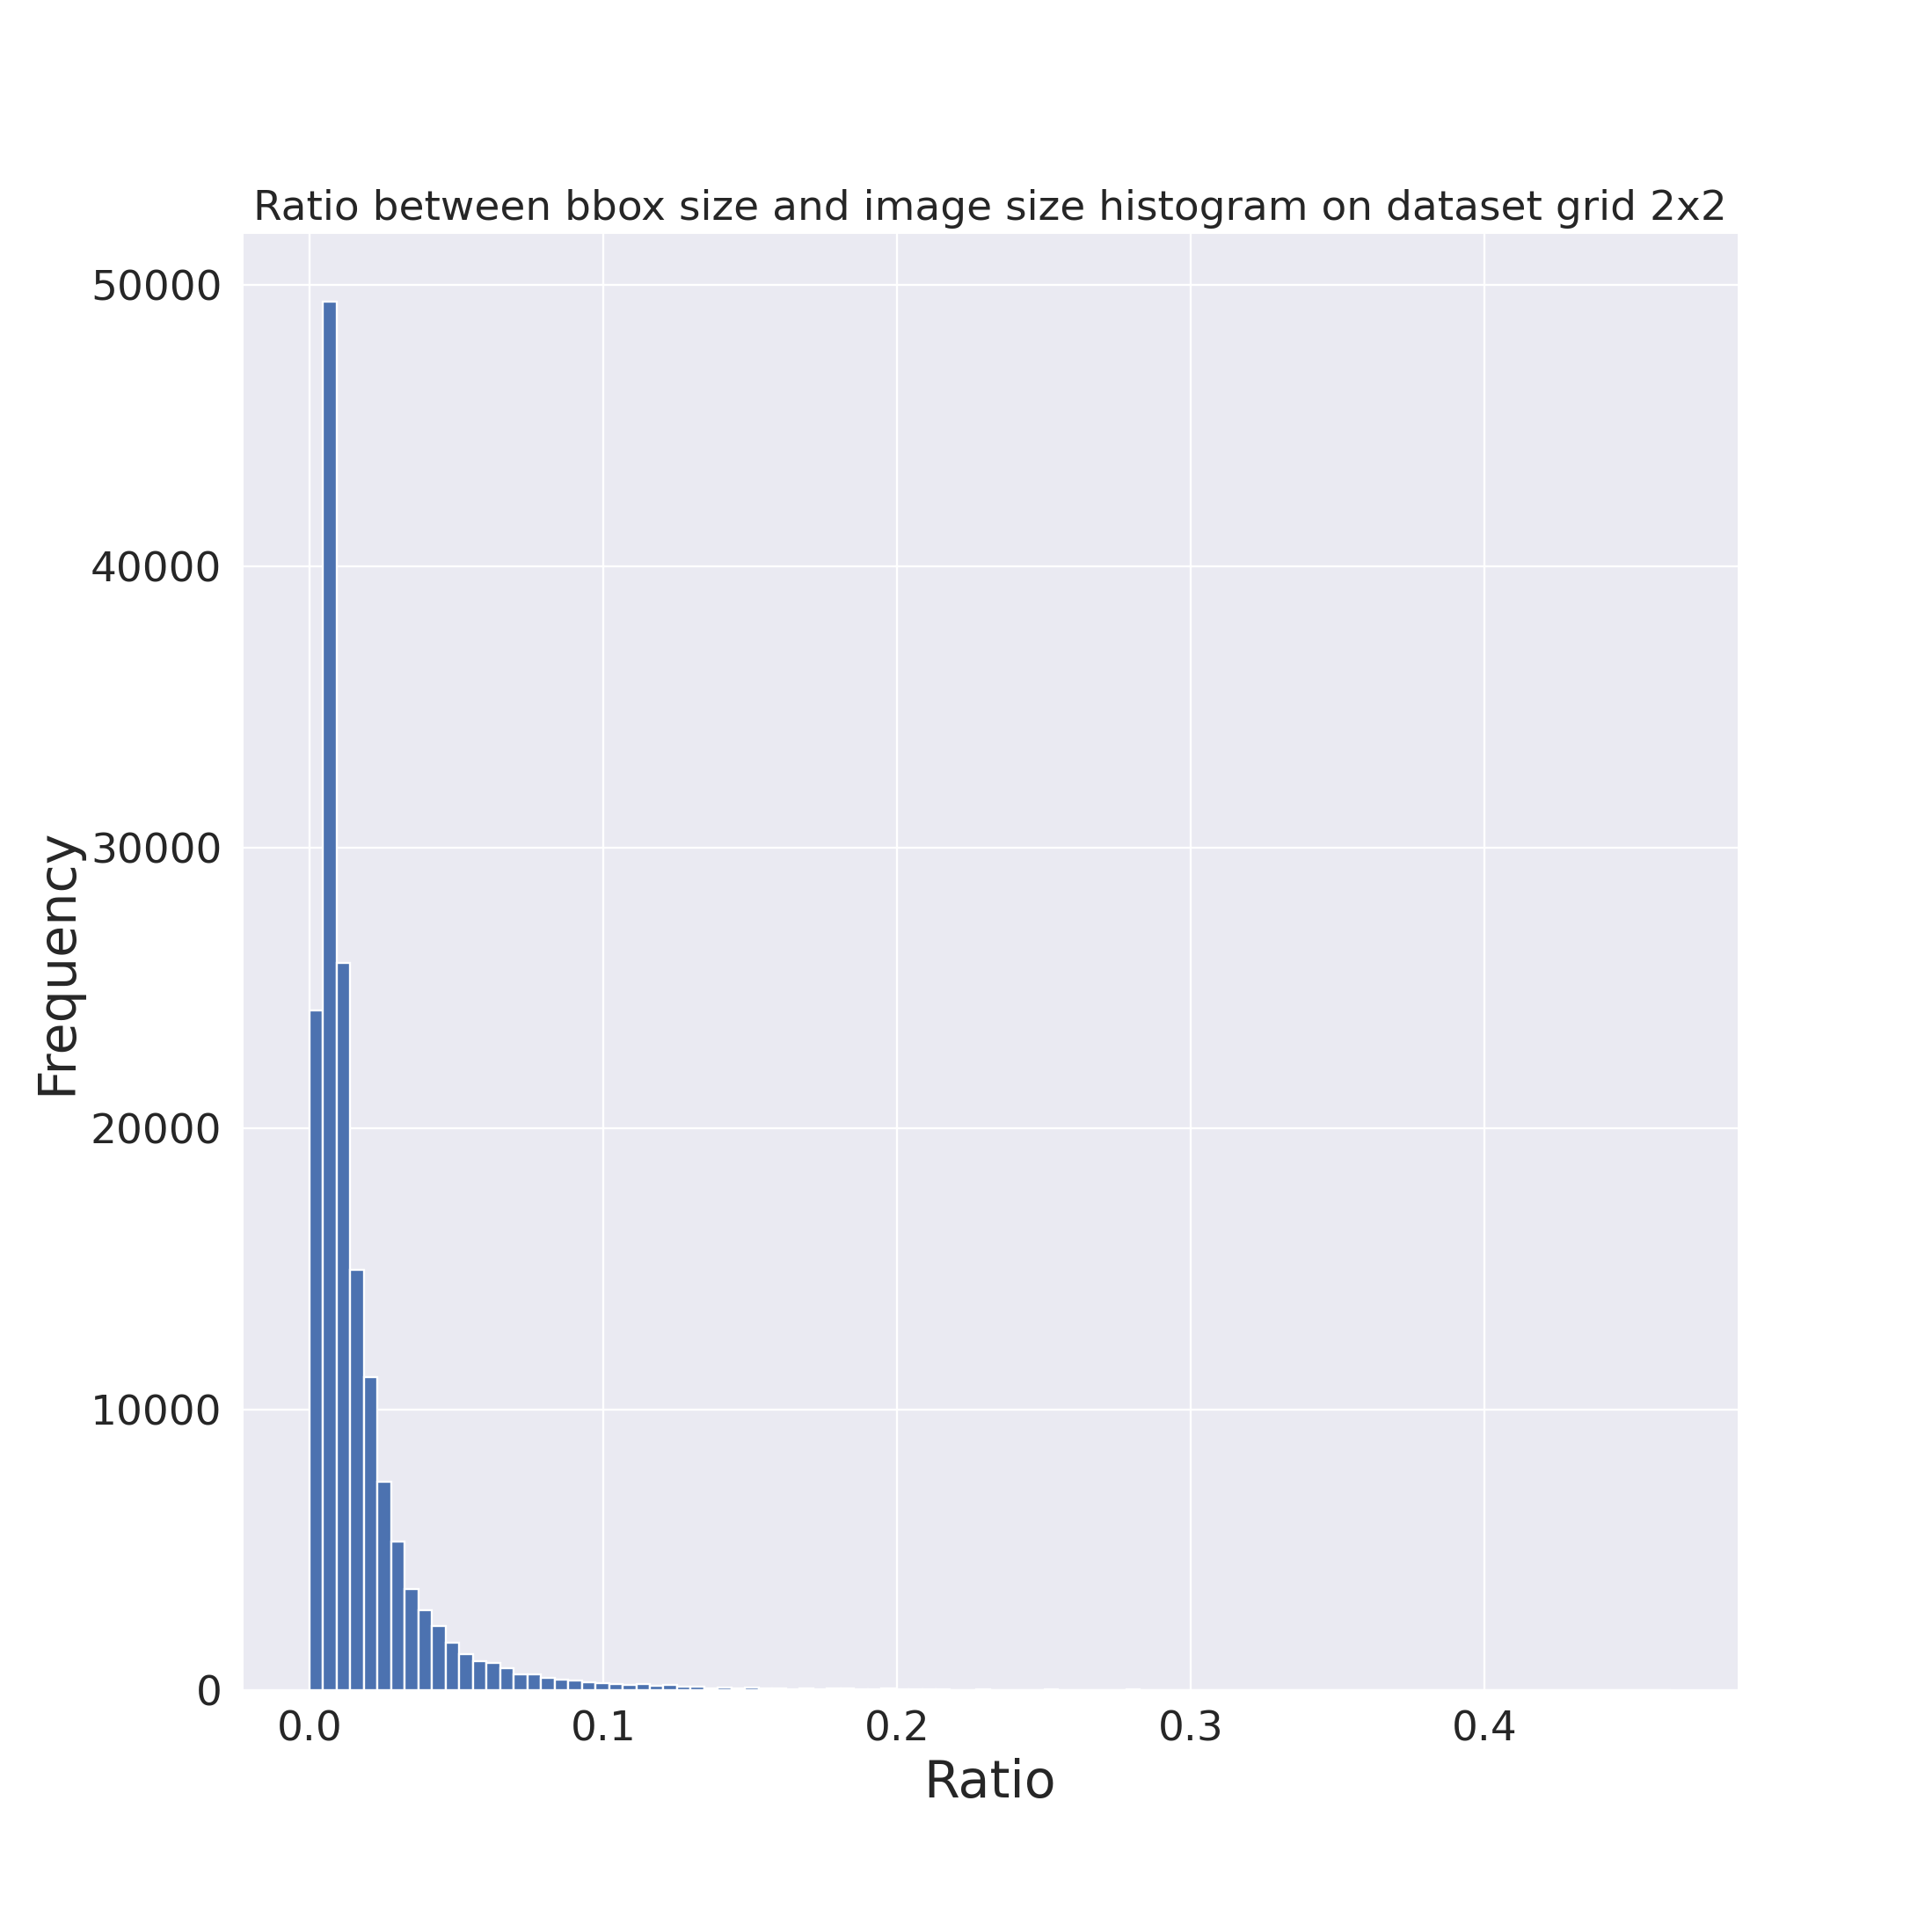
\includegraphics[width=7.3cm, trim={0.5cm 0.5cm 3cm 3cm}, clip]{images/widerface_nk_scale_2K}}
        \subfigure[]{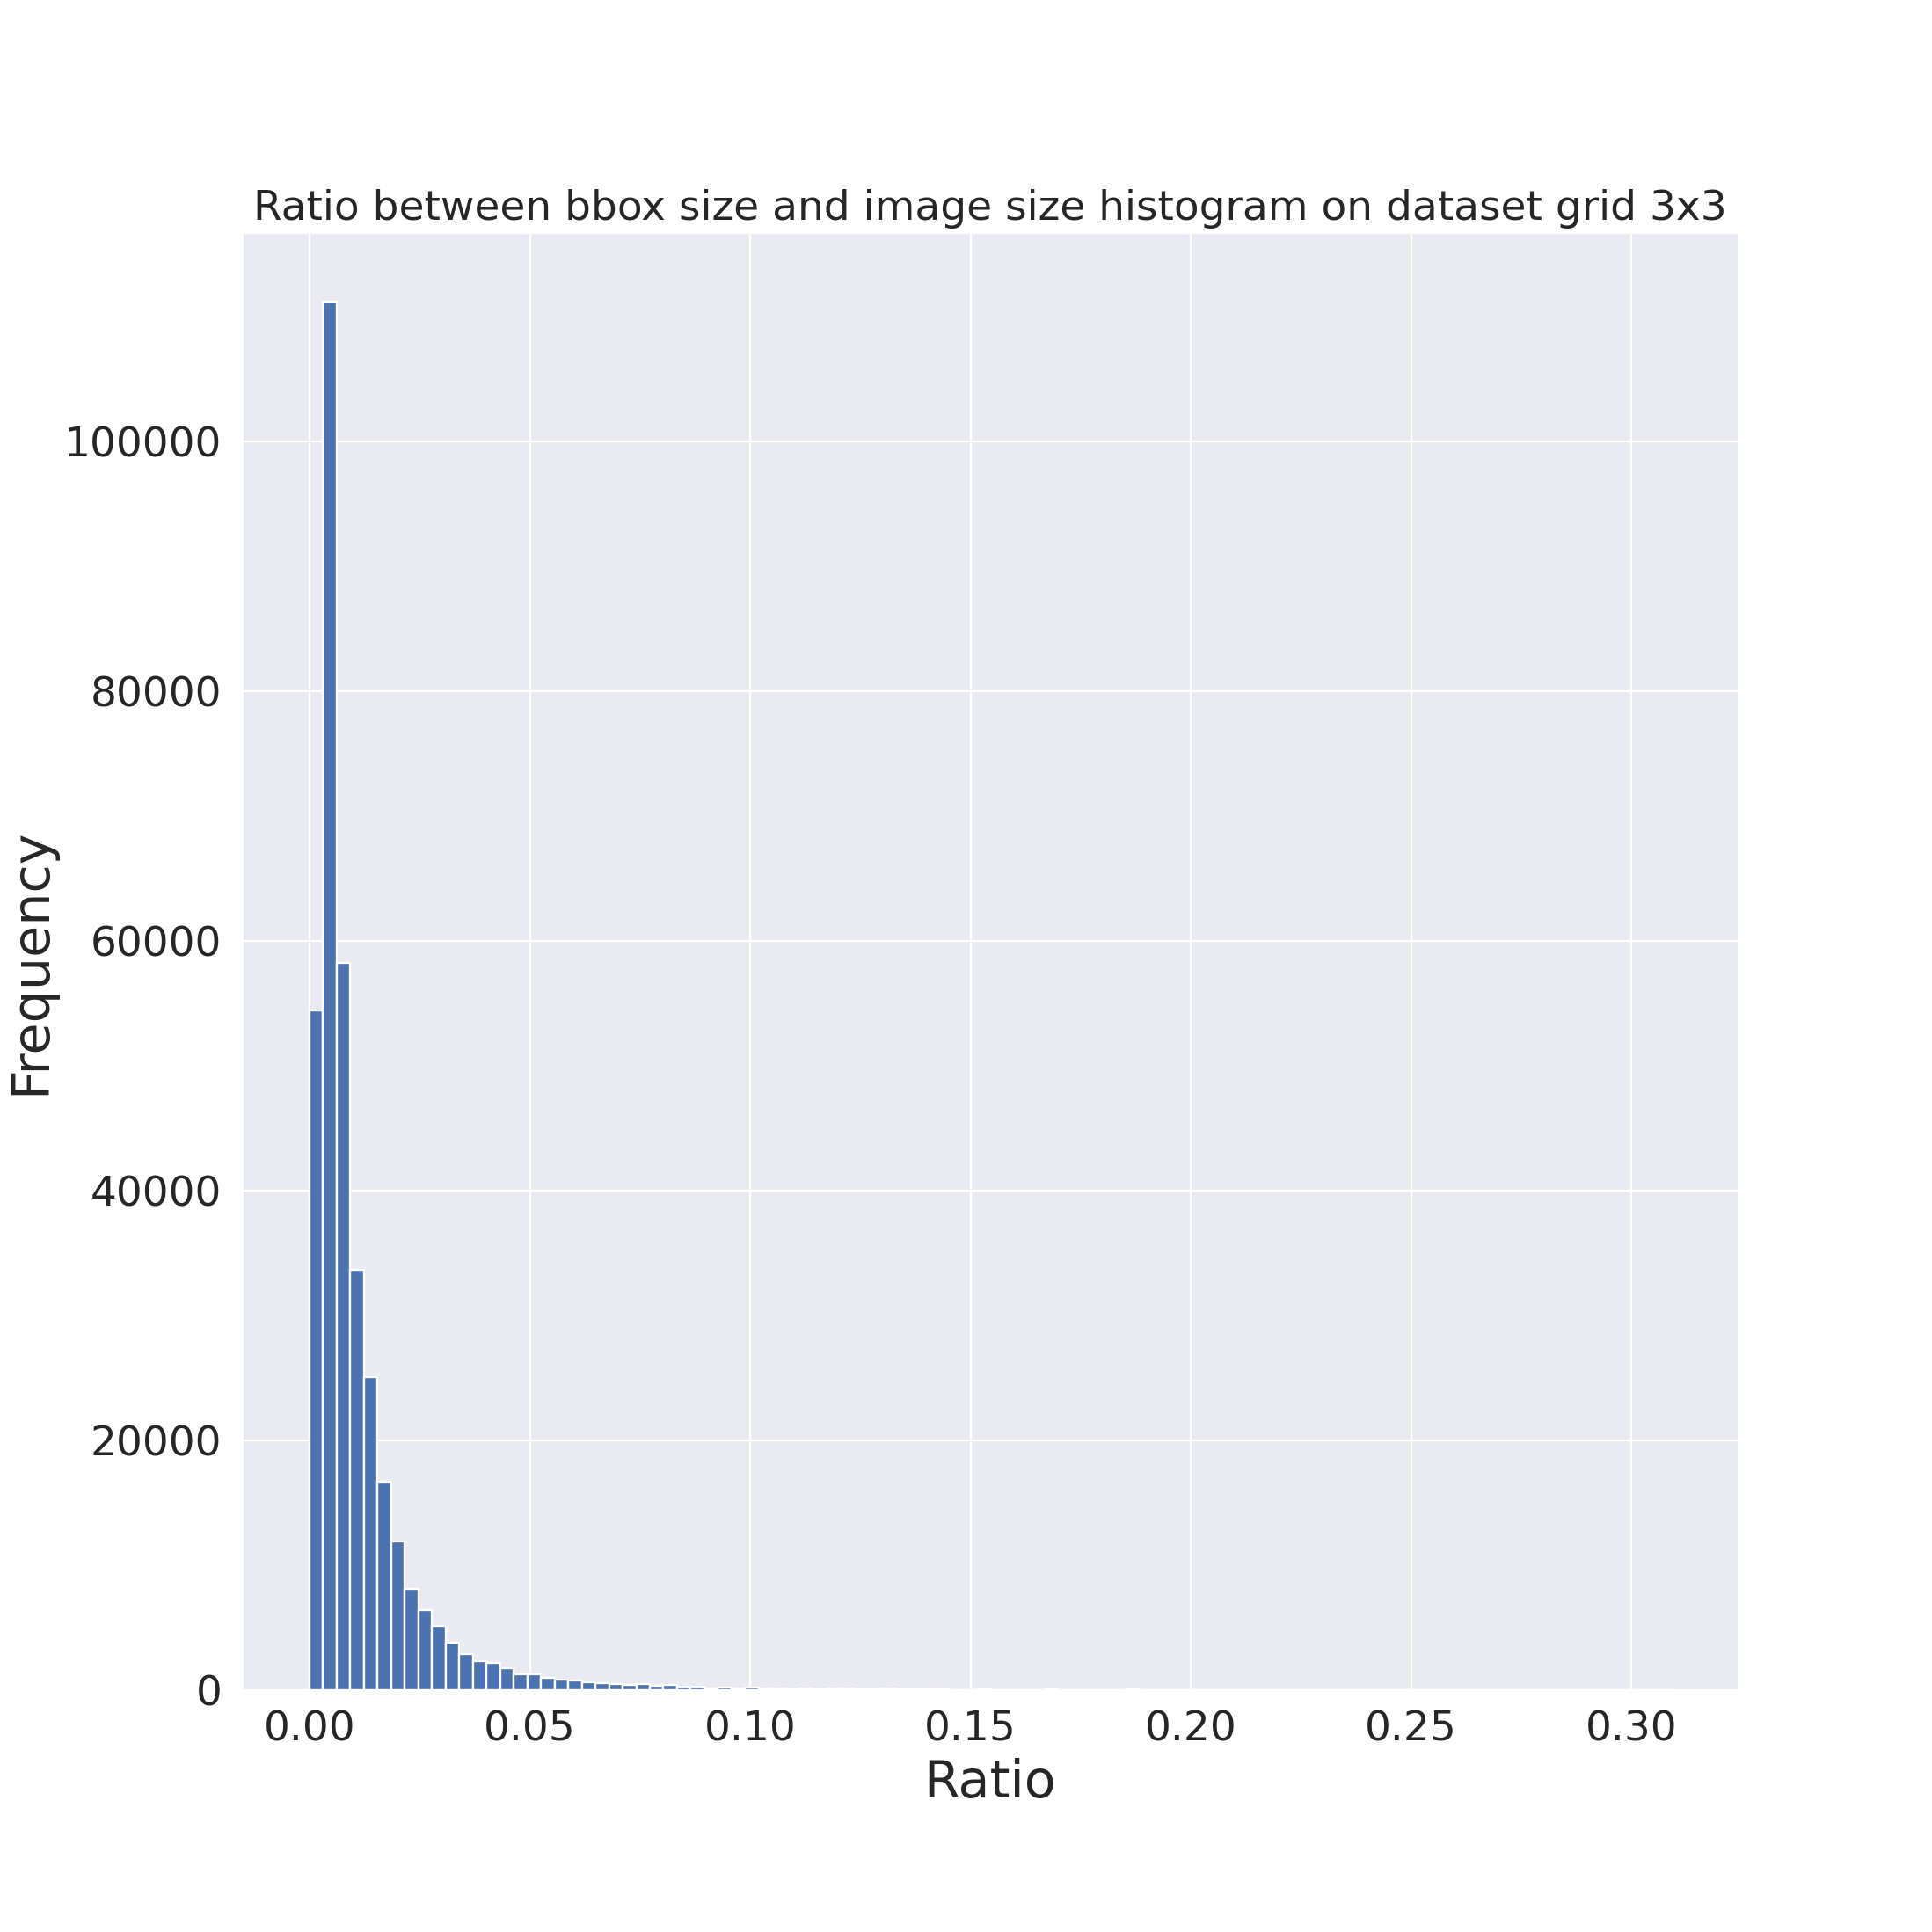
\includegraphics[width=7.3cm, trim={0.2cm 0.5cm 3cm 3cm}, clip]{images/widerface_nk_scale_3K}}
        \caption{Phân phối về tỷ lệ giữa kích thước của hộp giới hạn và kích thước ảnh trong bộ dữ liệu WIDER FACE \cite{yang2016wider} (a) so sánh với bộ dữ liệu WIDER FACE kích thước lớn dạng lưới $2 X 2$ (b) và $3 X 3$ (c)}
        \label{fig:widerface_4k_scale}
    \end{figure}

    \noindent
    Với việc kích thước ảnh được tăng lên đáng kể, việc nhận diện các khuôn mặt trong ảnh trở nên khó khăn hơn, đặc biệt là với các khuôn mặt có kích thước nhỏ.
    Trong bộ dữ liệu WIDER FACE kích thước lớn, số lượng các mặt có kích thước nhỏ so sánh tỷ lệ với kích thước ảnh trong bộ dữ liệu lớn hơn.
    Cụ thể, đối với bộ dữ liệu WIDER FACE, trung bình kích thước hộp giới hạn của khuôn mặt bằng khoảng 2\% kích thước của ảnh.

    \noindent
    Đối với bộ dữ liệu WIDER FACE kích thước lớn, trung bình kích thước hộp giới hạn của khuôn mặt bằng khoảng 1\% kích thước của ảnh đối với dạng lưới $2 X 2$ và 0.6\% kích thước của ảnh đối với dạng lưới $3 X 3$.

    \noindent
    Với những thông số trên, bộ dữ liệu WIDER FACE kích thước lớn được kỳ vọng giúp đánh giá khách quan độ chính xác và tốc độ của các mô hình giải bài toán nhận diện khuôn mặt với ảnh chất lượng cao.
}
    \widerfacefourk

    \subsection{Các thí nghiệm và kết quả của mô hình RetinaFocus}
    \def\retinafocusresults{
    Một đặc điểm của mô hình RetinaFocus là có nhiều cấu hình có thể cài đặt để triển khai mô hình như cấu hình lựa chọn feature maps \index{feature maps} của FPN cho Nhánh Focus \index{nhánh Focus}, cấu hình scale ảnh trong quá trình predict \dots
    Vì vậy, ta cần so sánh và lựa chọn cấu hình tối ưu nhất, cân đối giữa thời gian thực hiện quá trình predict và độ chính xác của mô hình.
    Để so sánh một cách toàn diện nhất, ta sẽ sử dụng cả hai bộ dữ liệu WIDER FACE thông thường và bộ dữ liệu WIDER FACE 4K đã được giới thiệu ở \textbf{\textit{phần 5.2}}.

    \noindent
    \textbf{\textit{Thí nghiệm so sánh cấu hình sử dụng feature maps \index{feature maps} khác nhau của FPN làm đầu vào cho Nhánh Focus}} \index{nhánh Focus} \\
    Trong thí nghiệm này, với mỗi cấu hình, chúng tôi sử dụng các feature maps \index{feature maps} khác nhau của FPN làm đầu vào cho Nhánh Focus \index{nhánh Focus}.
    Trong đó, lần lượt các cấu hình sử dụng feature maps \index{feature maps} ${C}_{3}, {C}_{4}, {C}_{5}, {P}_{3}, {P}_{4}, {P}_{5}$ được ký hiệu là \textit{C3}, \textit{C4}, \textit{C5}, \textit{P3}, \textit{P4}, \textit{P5} trong các biểu đồ.
    Trong các cấu hình trên, các cặp feature maps \index{feature maps} ${C}_{3}$ và ${P}_{3}$, ${C}_{4}$ và ${P}_{4}$, ${C}_{5}$ và ${P}_{5}$ là các cặp feature maps \index{feature maps} có cùng kích thước.
    Tuy nhiên, mỗi feature maps \index{feature maps} khác nhau trong cặp chứa thông tin khác nhau về khuôn mặt dẫn đến số lượng và kích thước của các vùng mà Nhánh Focus \index{nhánh Focus} xác định cần phải zoom vào cũng khác nhau.
    Từ đó dẫn đến thời gian thực hiện toàn bộ quá trình predict trên cả bộ dữ liệu là khác nhau.
    Trong thí nghiệm này, các cấu hình sử dụng chung một cấu hình scale ảnh trong quá trình predict là ....

    \begin{figure}[H]
        \centering
        \subfigure[]{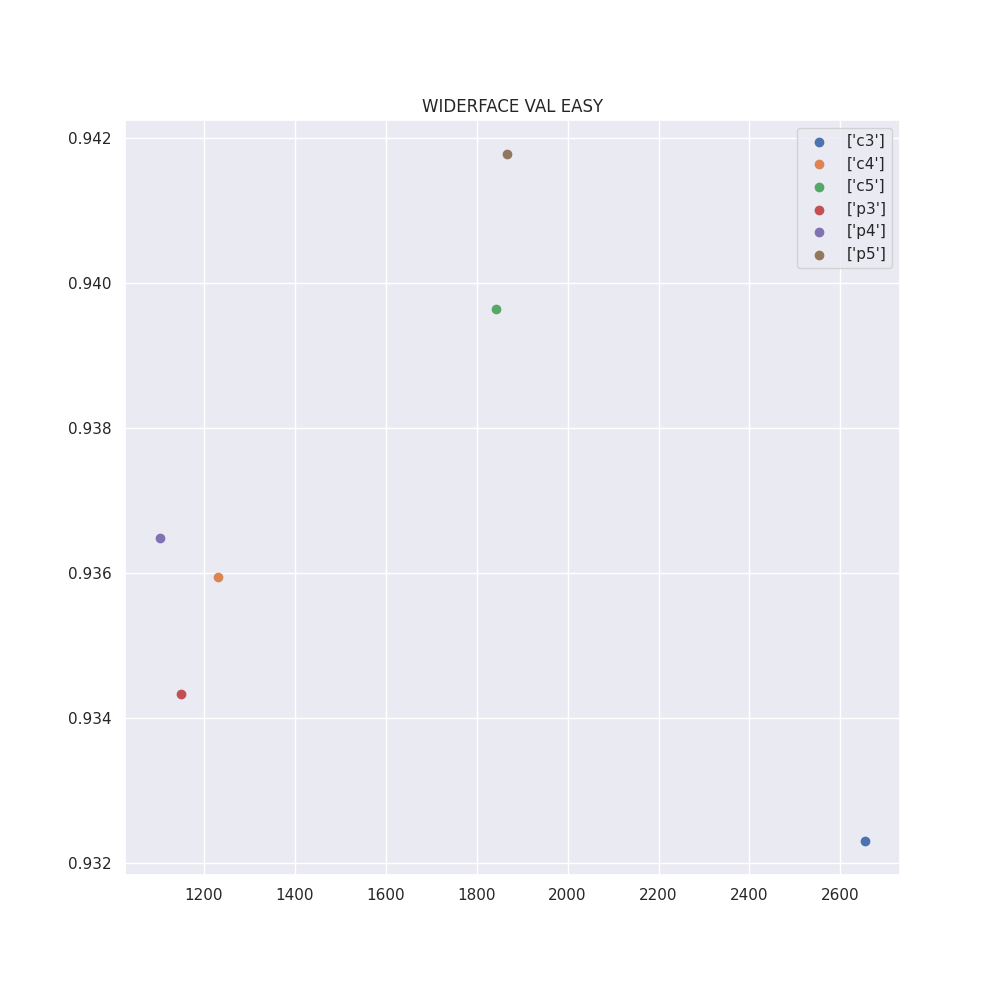
\includegraphics[width=0.32\textwidth, trim={2.3cm 2.3cm 2.3cm 2.3cm}, clip]{images/retinafocus_widerface_val_easy_fpn}} 
        \subfigure[]{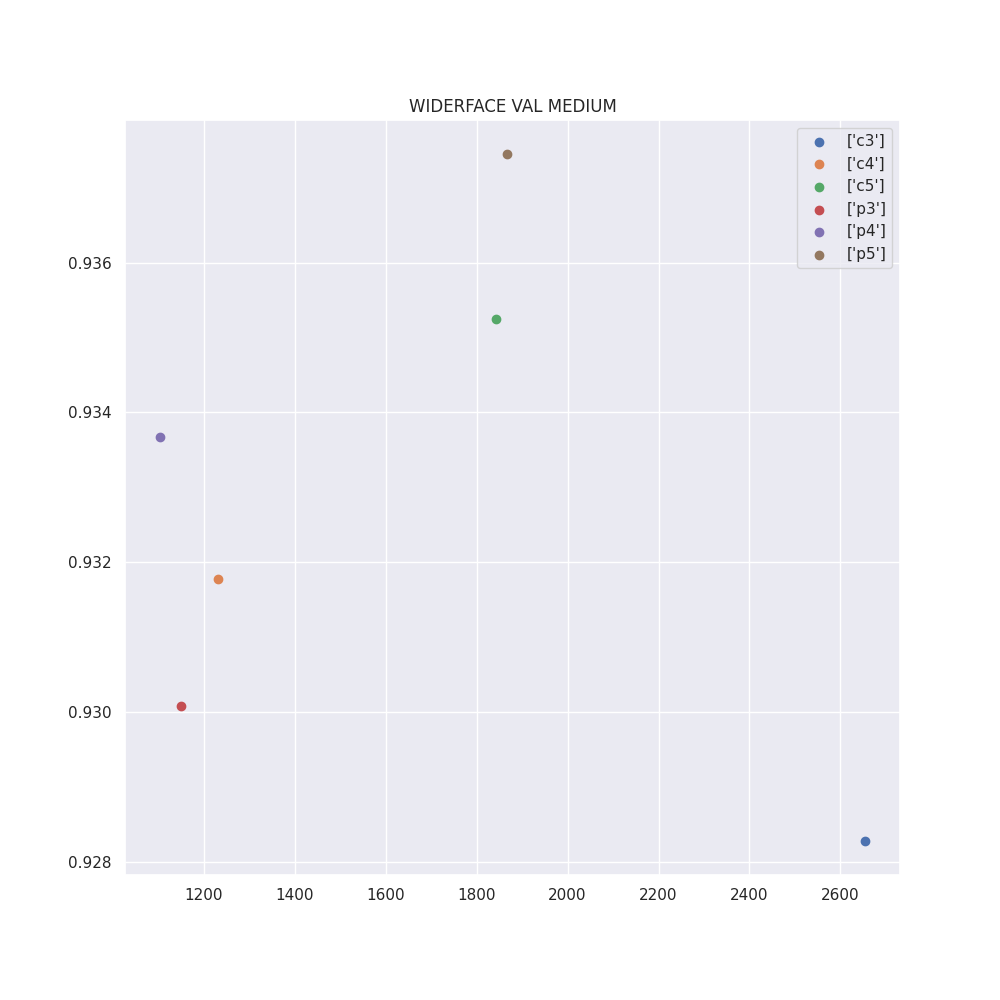
\includegraphics[width=0.32\textwidth, trim={2.3cm 2.3cm 2.3cm 2.3cm}, clip]{images/retinafocus_widerface_val_medium_fpn}} 
        \subfigure[]{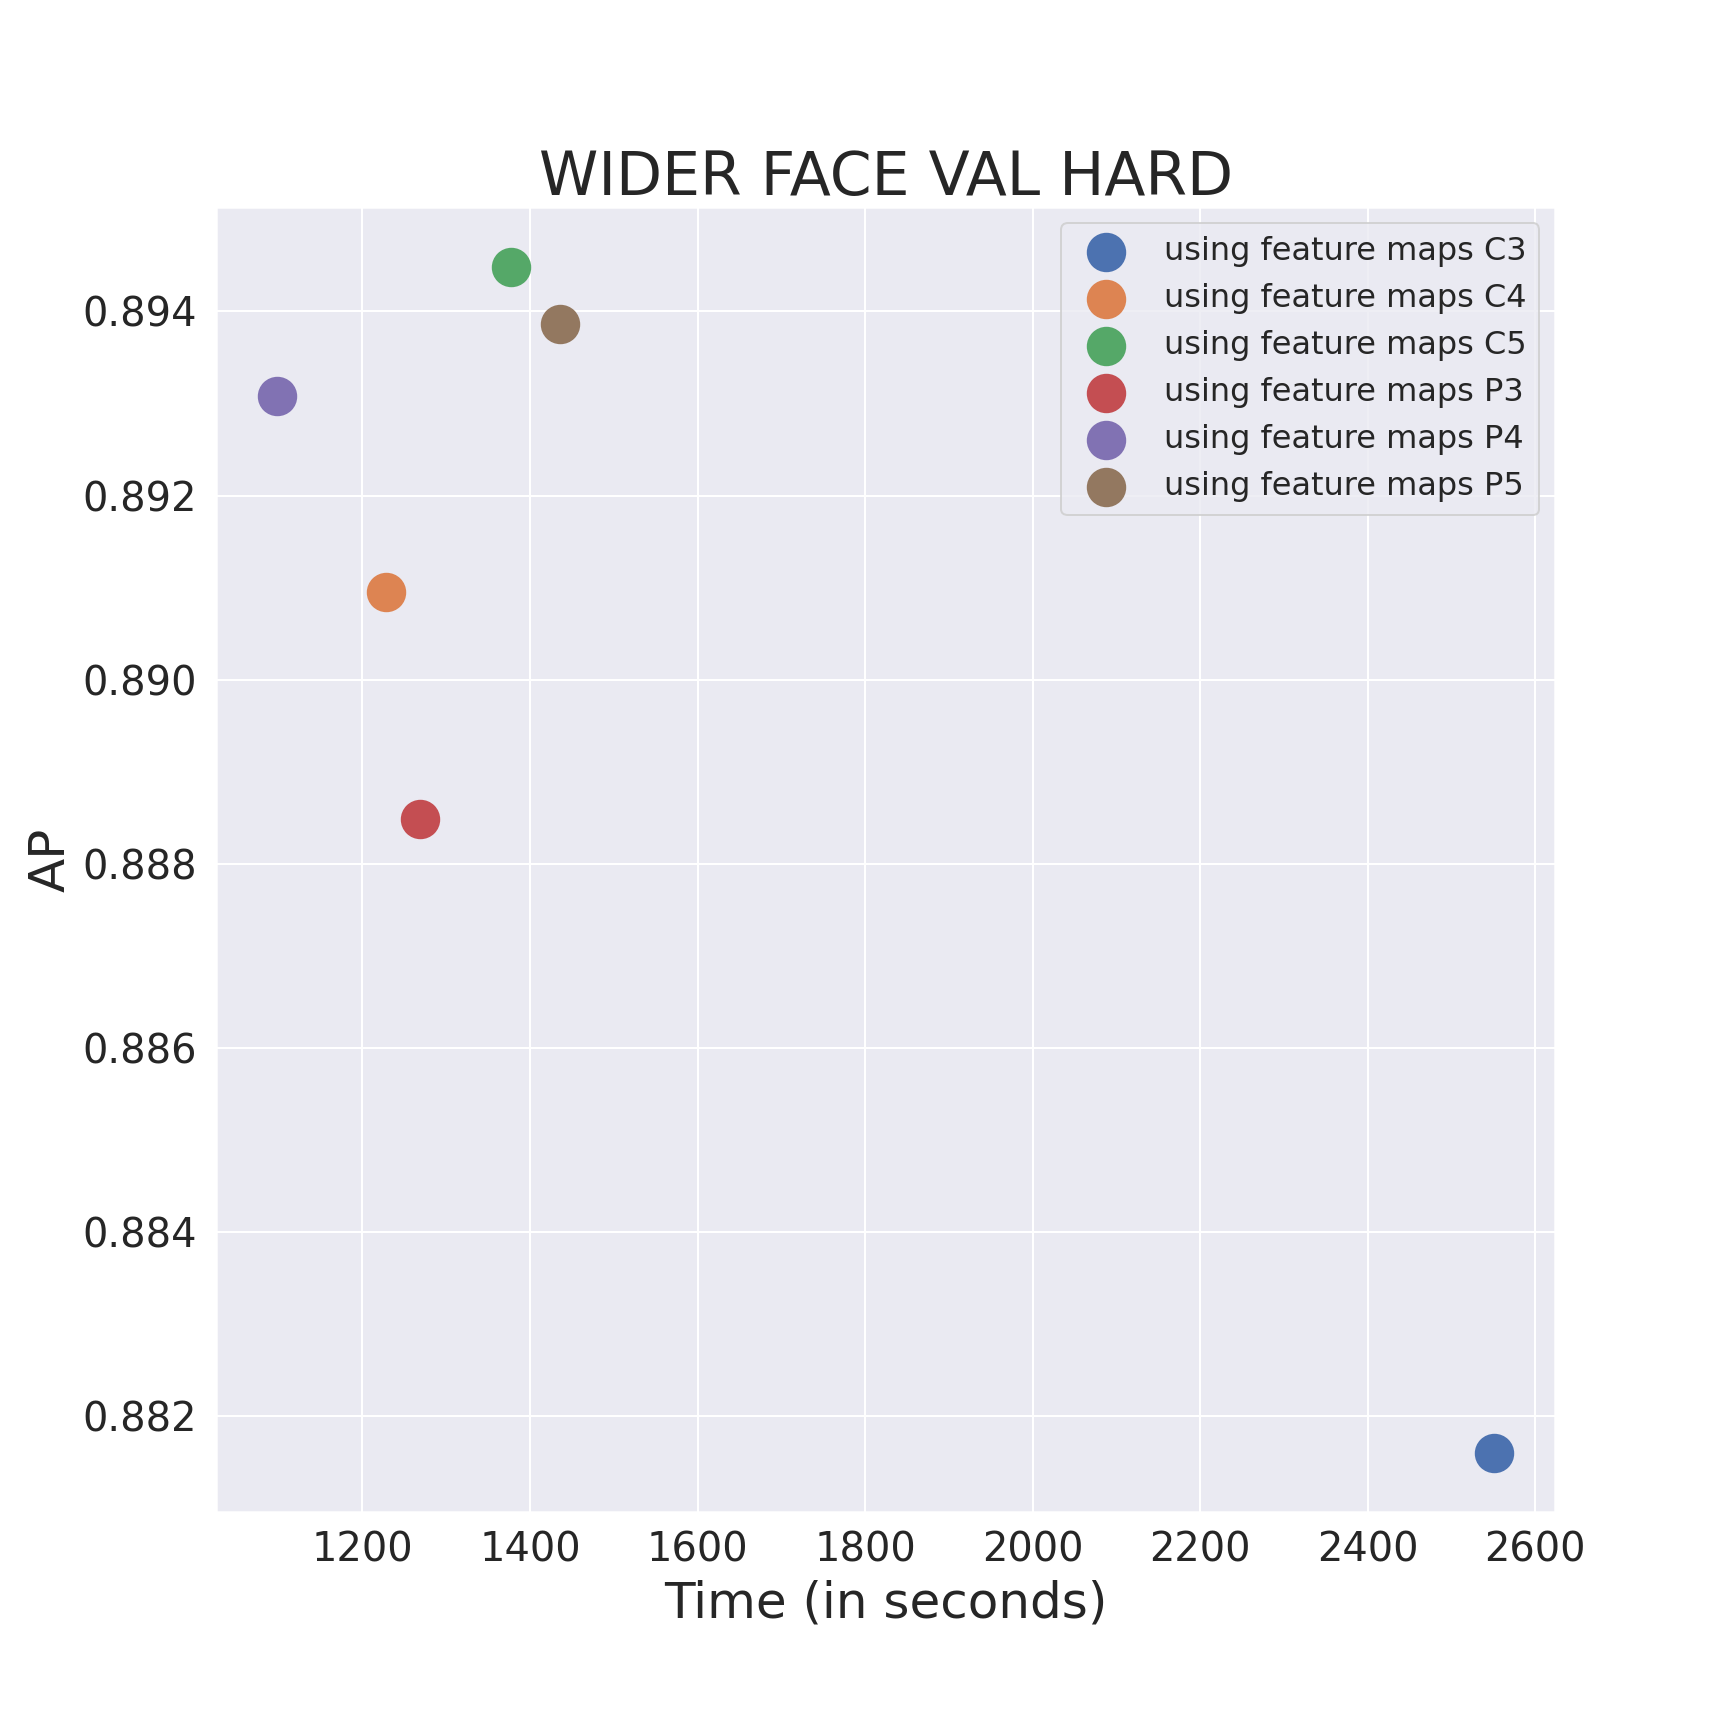
\includegraphics[width=0.32\textwidth, trim={2.3cm 2.3cm 2.3cm 2.3cm}, clip]{images/retinafocus_widerface_val_hard_fpn}} 
        \caption{Kết quả so sánh các cấu hình sử dụng các feature maps \index{feature maps} của FPN làm đầu vào cho Nhánh Focus \index{nhánh Focus} trên ba bộ dữ liệu WIDER FACE val easy (a), medium (b) và hard (c)}
        \label{fig:retinafocus_widerface_val_fpn}
    \end{figure}

    \noindent
    Đối với bộ WIDER FACE thông thường, hai cấu hình đạt độ chính xác cao nhất là cấu hình sử dụng feature maps \index{feature maps} ${P}_{5}$ và cấu hình sử dụng feature maps \index{feature maps} ${C}_{5}$ cho Nhánh Focus \index{nhánh Focus} với thời gian thực hiện toàn bộ quá trình predict trên cả bộ dữ liệu lần lượt là ... và ....
    Trong khi cấu hình sử dụng feature maps \index{feature maps} ${P}_{5}$ cho kết quả tốt hơn trên bộ WIDER FACE val easy và medium thì cấu hình sử dụng feature maps \index{feature maps} ${C}_{5}$ cho kết quả tốt hơn trên bộ WIDER FACE val hard.
    Các cấu hình khác như ${P}_{4}$, ${P}_{3}$ và ${C}_{4}$ có thời gian thực hiện toàn bộ quá trình predict nhanh hơn nhưng độ chính xác không tốt.
    Đặc biệt là cấu hình ${C}_{3}$ vừa có thời gian thực hiện toàn bộ quá trình predict chậm vừa đạt độ chính xác thấp.

    \begin{figure}[H]
        \centering
        \subfigure[]{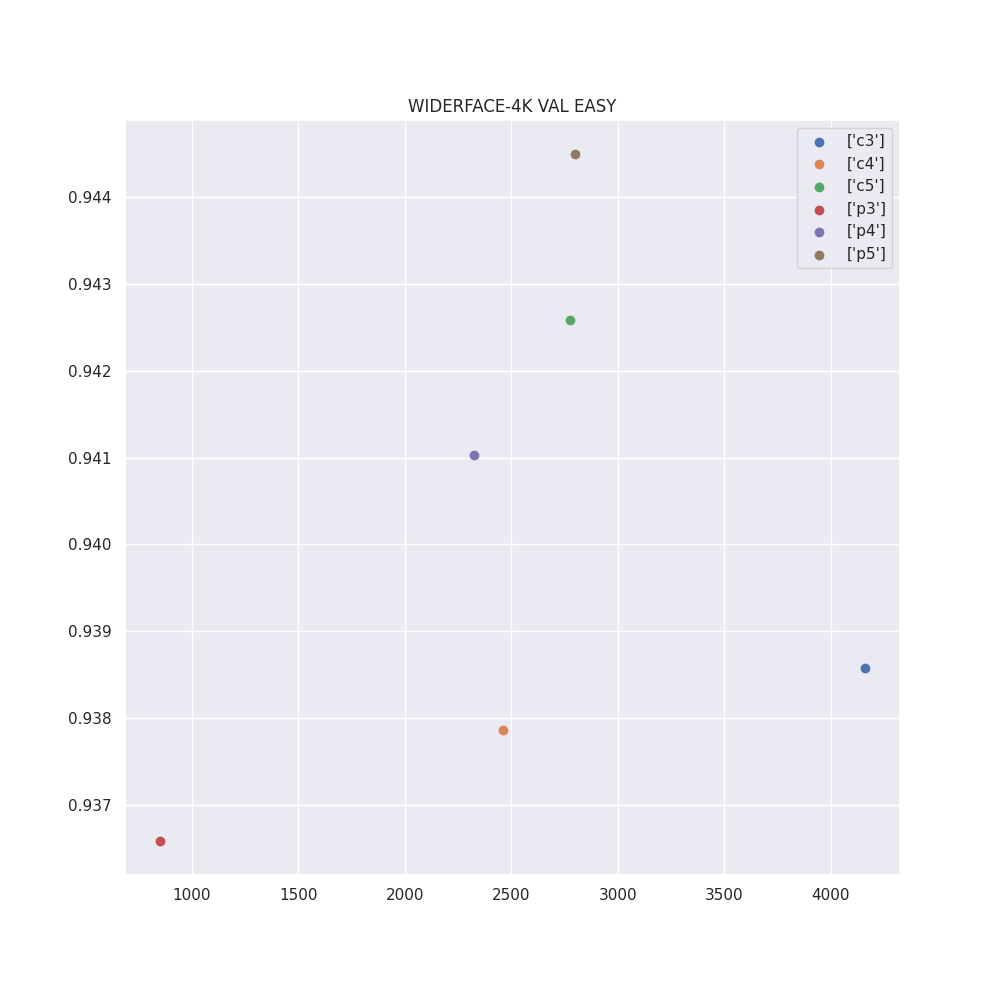
\includegraphics[width=0.32\textwidth, trim={2.3cm 2.3cm 2.3cm 2.3cm}, clip]{images/retinafocus_widerface_4k_val_easy_fpn}} 
        \subfigure[]{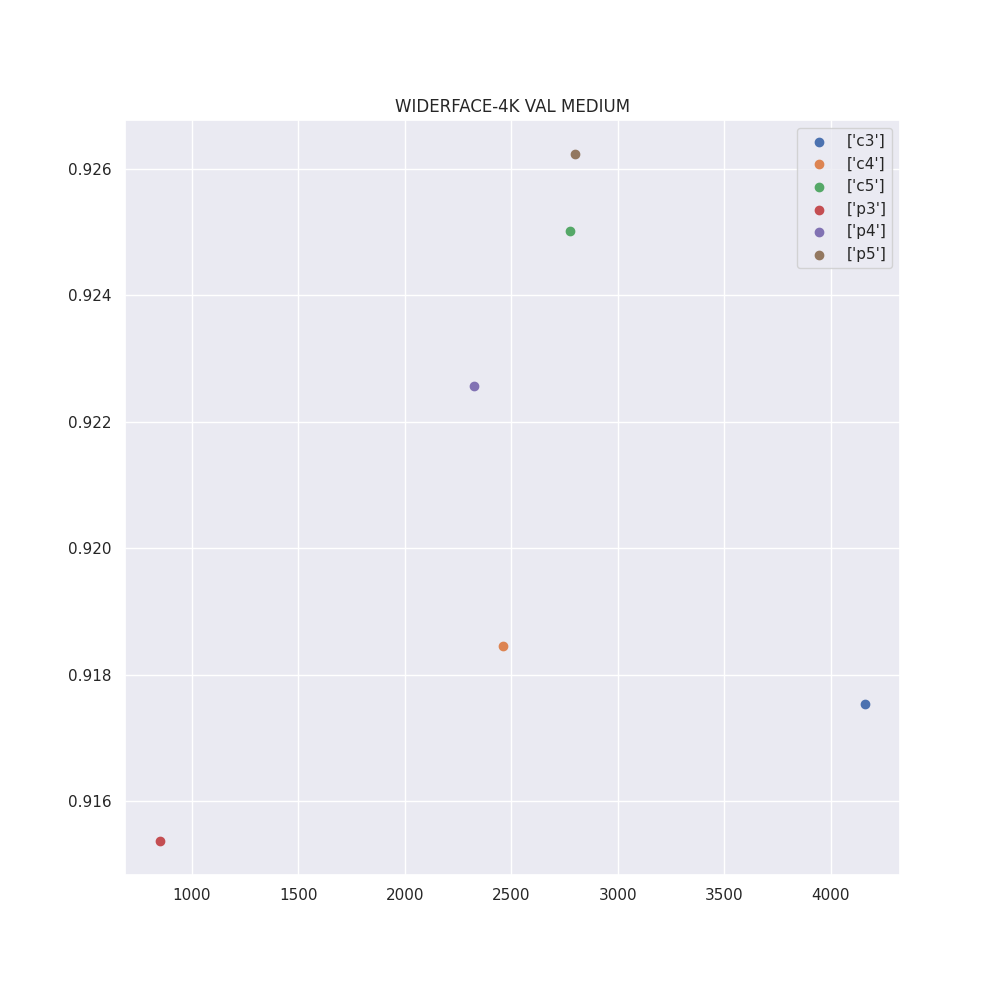
\includegraphics[width=0.32\textwidth, trim={2.3cm 2.3cm 2.3cm 2.3cm}, clip]{images/retinafocus_widerface_4k_val_medium_fpn}} 
        \subfigure[]{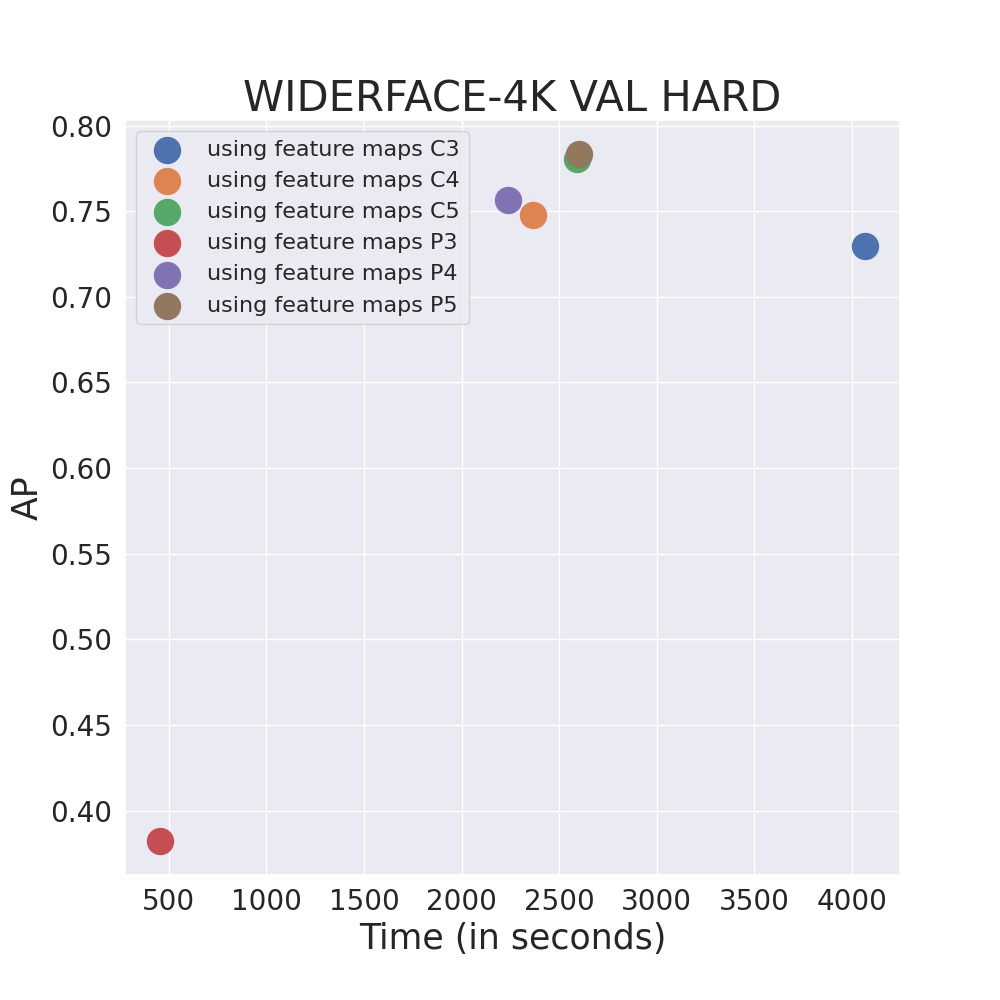
\includegraphics[width=0.32\textwidth, trim={2.3cm 2.3cm 2.3cm 2.3cm}, clip]{images/retinafocus_widerface_4k_val_hard_fpn}} 
        \caption{Kết quả so sánh các cấu hình sử dụng các feature maps \index{feature maps} của FPN làm đầu vào cho Nhánh Focus \index{nhánh Focus} trên ba bộ dữ liệu WIDER FACE 4K val easy (a), medium (b) và hard (c)}
        \label{fig:retinafocus_widerface_4k_val_fpn}
    \end{figure}

    \noindent
    Đối với bộ WIDER FACE 4K, hai cấu hình đạt độ chính xác cao nhất vẫn là cấu hình sử dụng feature maps \index{feature maps} ${P}_{5}$ và cấu hình sử dụng feature maps \index{feature maps} ${C}_{5}$ với thời gian thực hiện toàn bộ quá trình predict trên cả bộ dữ liệu lần lượt là ... và ....
    Đối với bộ dữ liệu này, cấu hình sử dụng feature maps \index{feature maps} ${P}_{5}$ cho kết quả tốt hơn so với cấu hình sử dụng feature maps \index{feature maps} ${C}_{5}$ trên cả ba bộ WIDER FACE 4K val easy, medium và hard.

    \noindent
    Kết luận đối với thí nghiệm này là cấu hình sử dụng feature maps \index{feature maps} ${P}_{5}$ đạt kết quả tốt nhất về độ chính xác trong khi vẫn duy trì được thời gian thực hiện toàn bộ quá trình predict tương đối nhanh.

    \noindent
    \textbf{\textit{Thí nghiệm so sánh cấu hình scale ảnh tốt nhất trong quá trình predict}} \\

    \noindent
    \textbf{\textit{Thí nghiệm so sánh cấu hình tốt nhất của RetinaFocus với các cấu hình của RetinaFace}} \\
    Các cấu hình của mô hình RetinaFace sử dụng trong thí nghiệm này bao gồm: \\
    - Cấu hình sử dụng chiến lược Image Pyramids kết hợp với việc lật ảnh đầu vào trong quá trình predict, ký hiệu là \dots \\
    - Cấu hình chỉ sử dụng chiến lược Image Pyramids, ký hiệu là \dots \\
    - Cấu hình không sử dụng chiến lược Image Pyramids mà chỉ sử dụng một scale ảnh duy nhất là [1200, 1600], ký hiệu là \dots \\
    - Cấu hình không sử dụng chiến lược Image Pyramids mà chỉ sử dụng một scale ảnh duy nhất là [1504, 2000], ký hiệu là \dots \\
    - Cấu hình không sử dụng chiến lược Image Pyramids mà chỉ sử dụng một scale ảnh duy nhất là [1600, 2150], ký hiệu là \dots \\

    \begin{figure}[H]
        \centering
        \subfigure[]{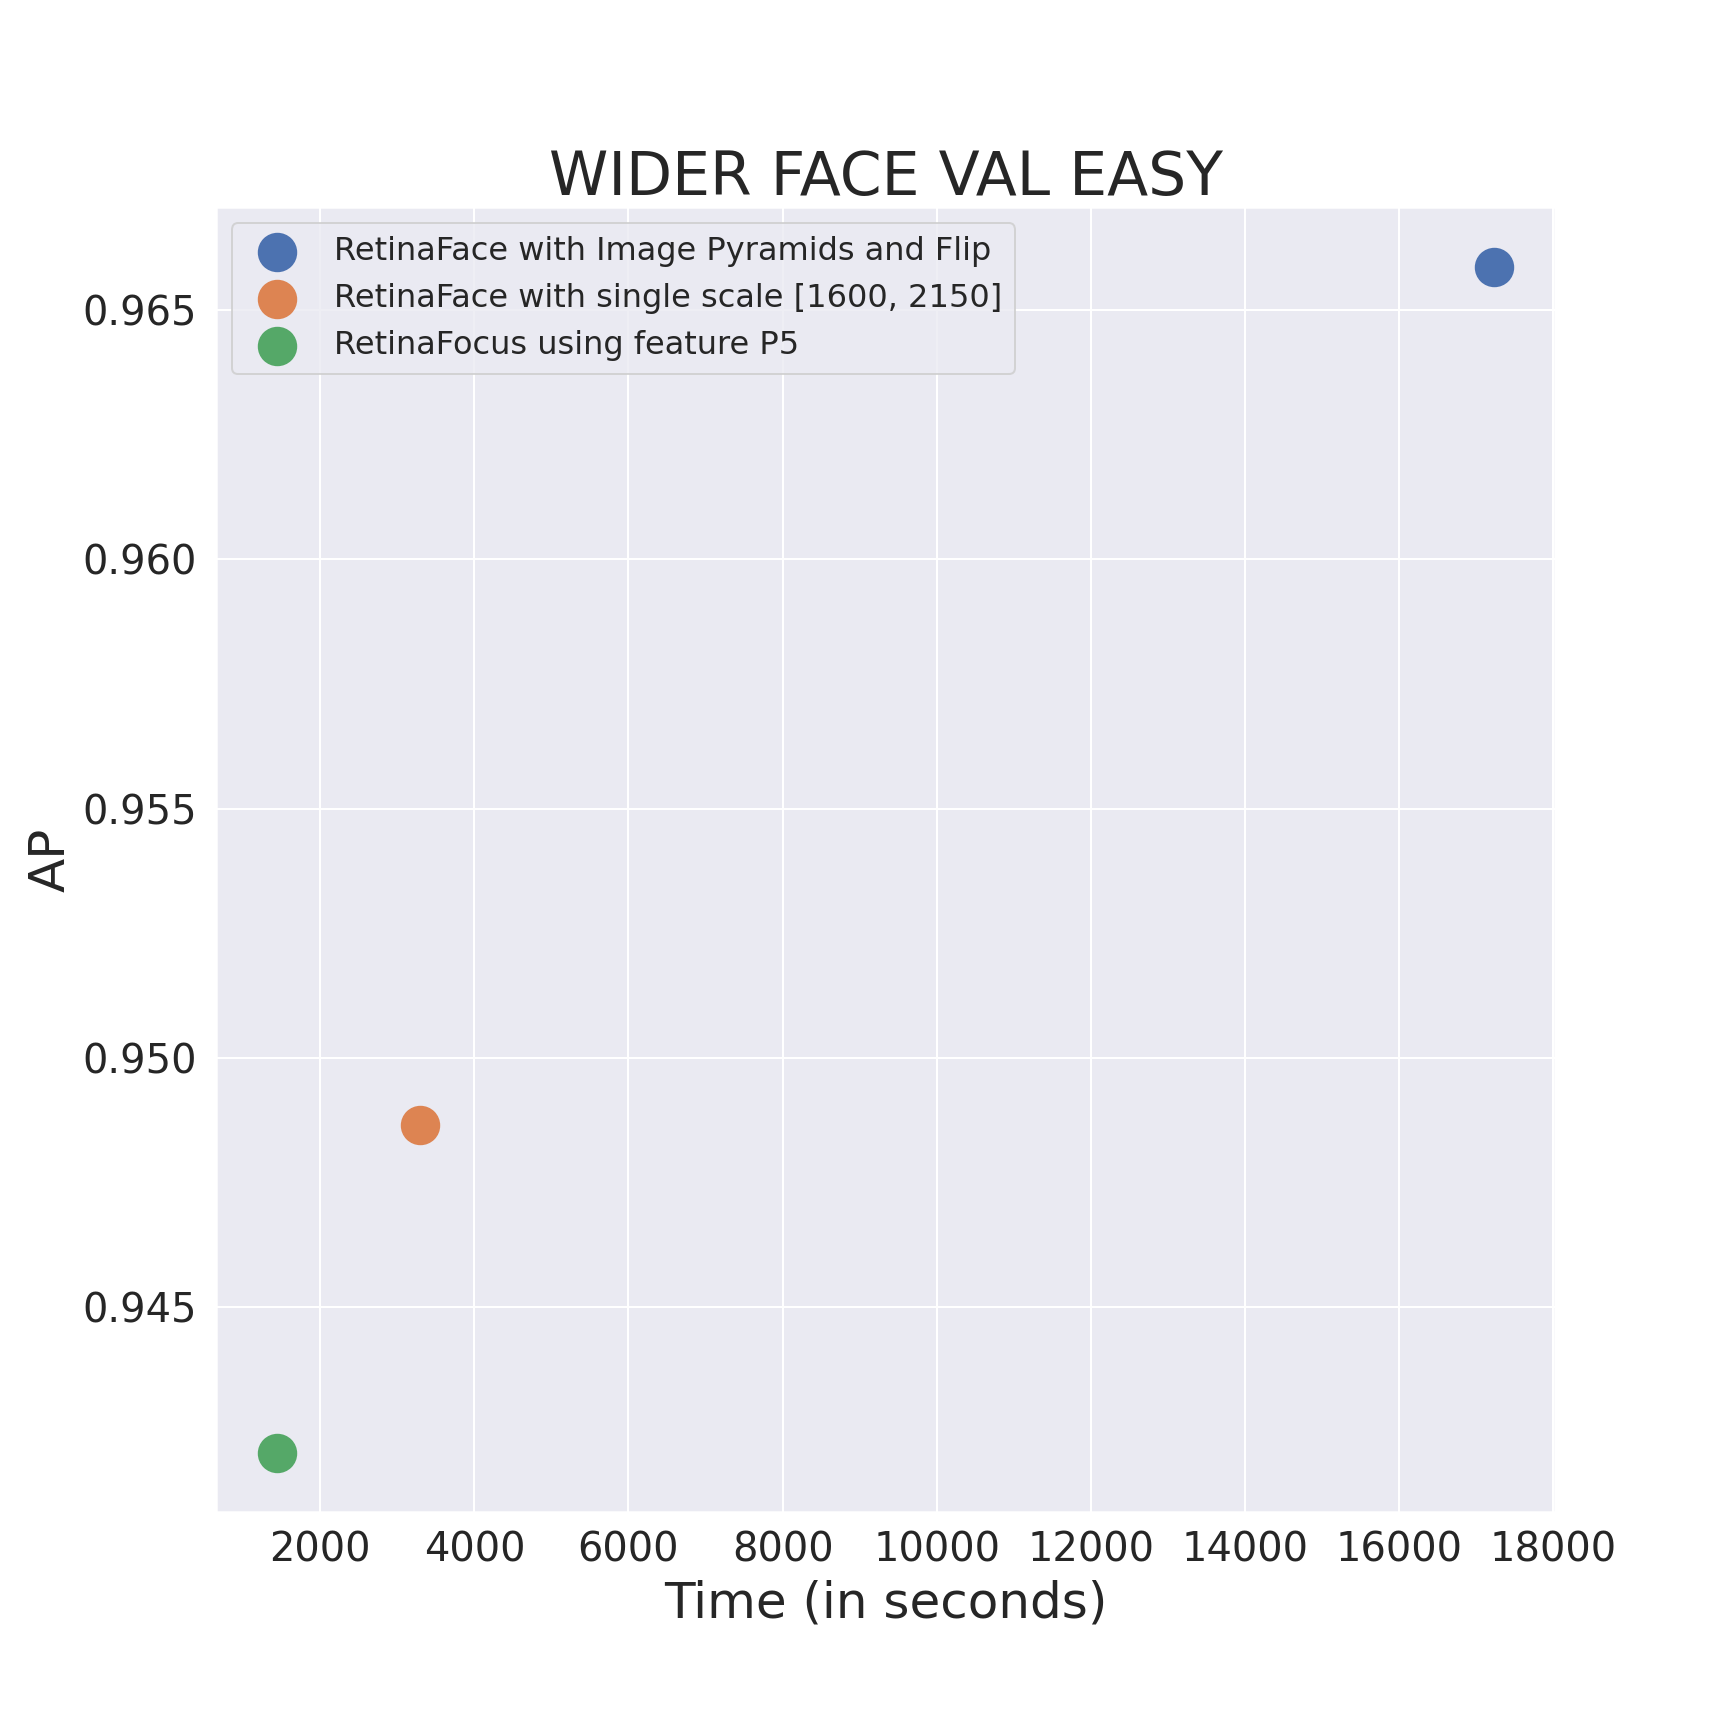
\includegraphics[width=0.32\textwidth, trim={2.3cm 2.3cm 2.3cm 2.3cm}, clip]{images/retinafocus_widerface_val_easy_rtnf}} 
        \subfigure[]{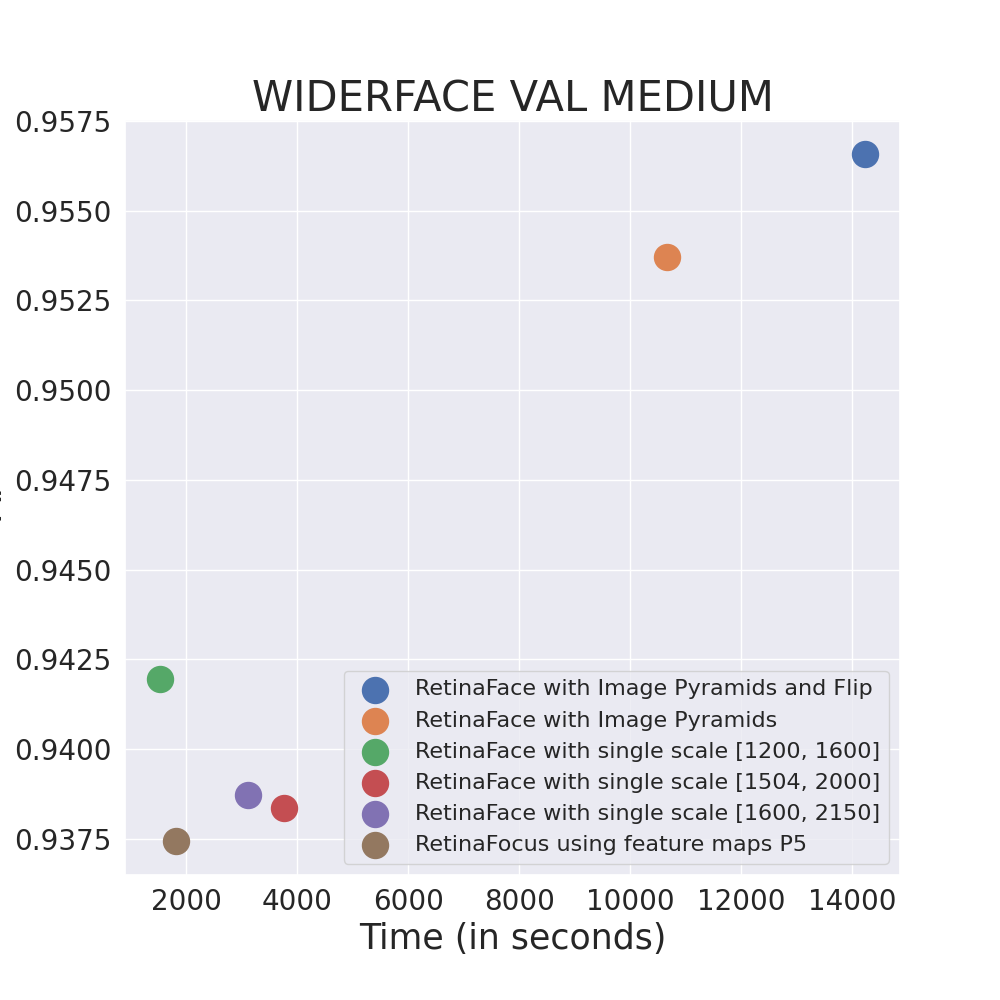
\includegraphics[width=0.32\textwidth, trim={2.3cm 2.3cm 2.3cm 2.3cm}, clip]{images/retinafocus_widerface_val_medium_rtnf}} 
        \subfigure[]{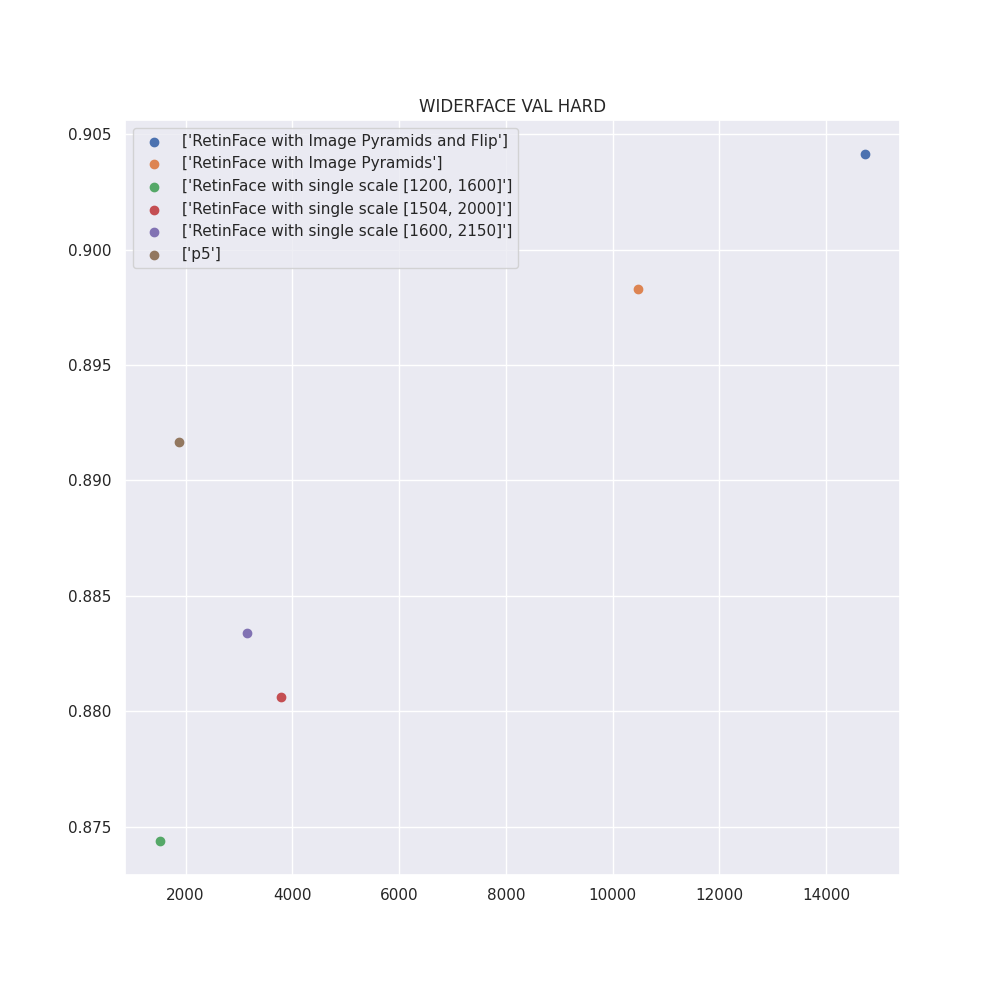
\includegraphics[width=0.32\textwidth, trim={2.3cm 2.3cm 2.3cm 2.3cm}, clip]{images/retinafocus_widerface_val_hard_rtnf}} 
        \caption{Kết quả so sánh cấu hình tốt nhất của RetinaFocus với các cấu hình của RetinaFace trên ba bộ dữ liệu WIDER FACE val easy (a), medium (b) và hard (c)}
        \label{fig:retinafocus_widerface_val_rtnf}
    \end{figure}

    \begin{figure}[H]
        \centering
        \subfigure[]{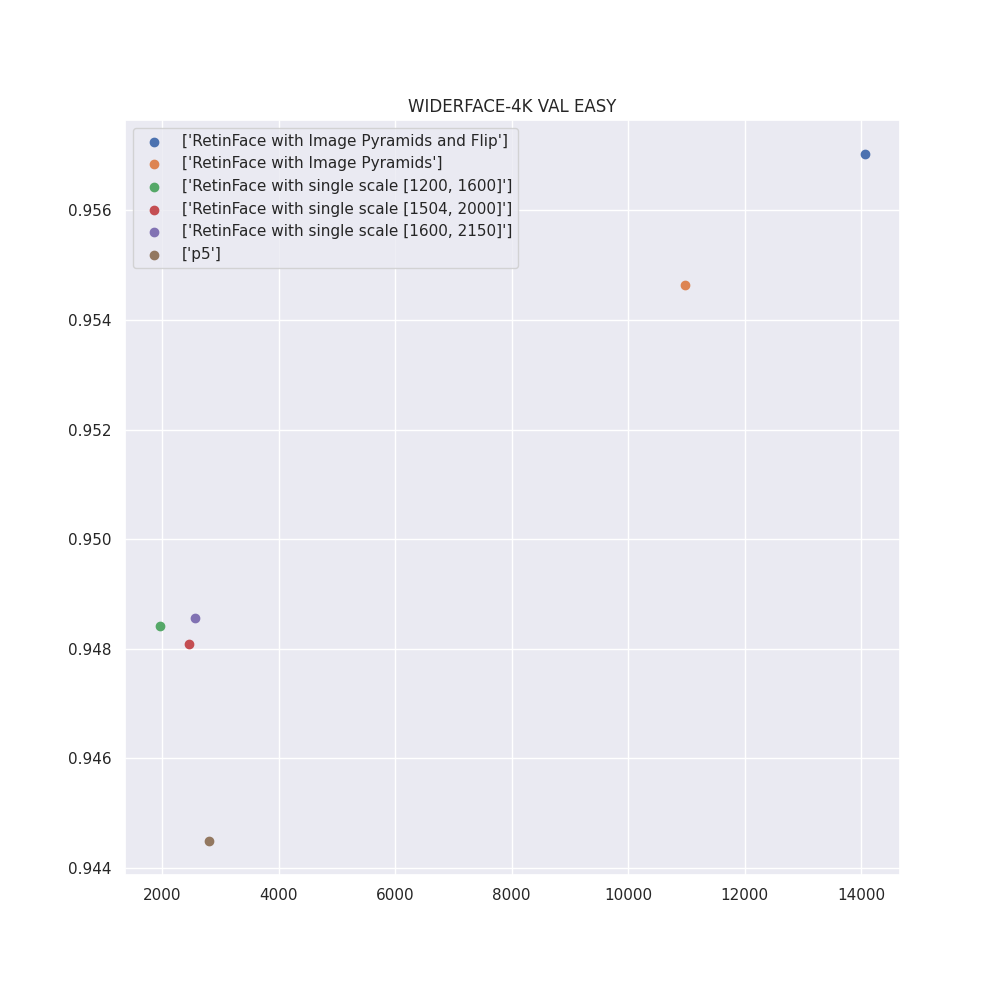
\includegraphics[width=0.32\textwidth, trim={2.3cm 2.3cm 2.3cm 2.3cm}, clip]{images/retinafocus_widerface_4k_val_easy_rtnf}} 
        \subfigure[]{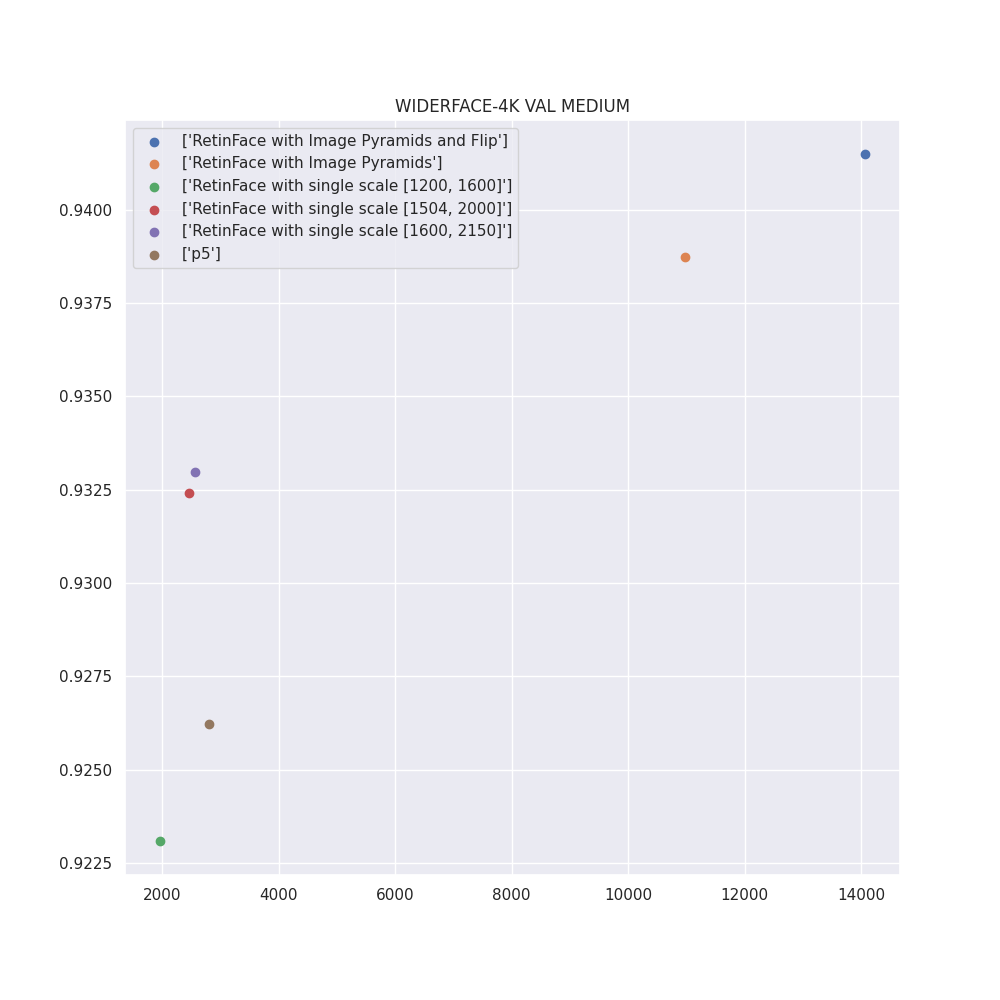
\includegraphics[width=0.32\textwidth, trim={2.3cm 2.3cm 2.3cm 2.3cm}, clip]{images/retinafocus_widerface_4k_val_medium_rtnf}} 
        \subfigure[]{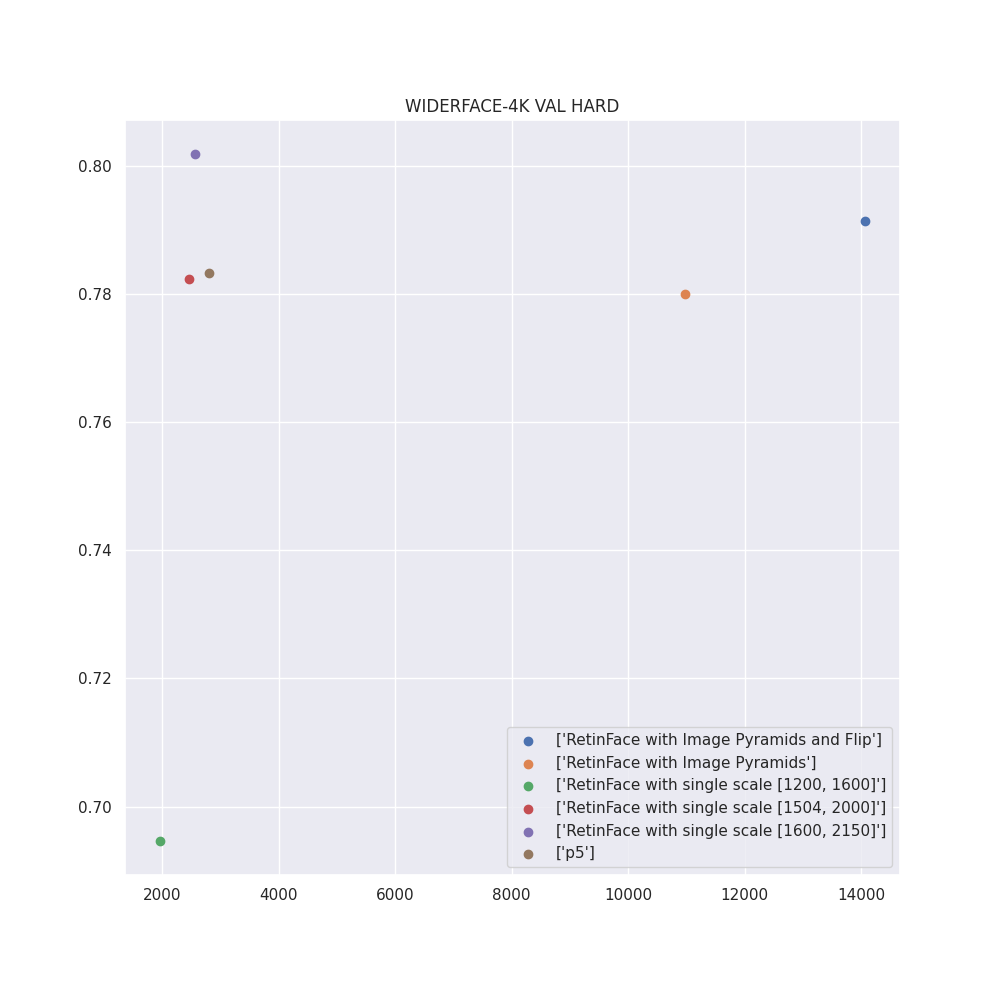
\includegraphics[width=0.32\textwidth, trim={2.3cm 2.3cm 2.3cm 2.3cm}, clip]{images/retinafocus_widerface_4k_val_hard_rtnf}} 
        \caption{Kết quả so sánh cấu hình tốt nhất của RetinaFocus với các cấu hình của RetinaFace trên ba bộ dữ liệu WIDER FACE 4K val easy (a), medium (b) và hard (c)}
        \label{fig:retinafocus_widerface_val_rtnf}
    \end{figure}

}
    \retinafocusresults

}
